\documentclass[12pt, a4paper, oneside]{book}   	% document style definition


\usepackage{hslu}                               % apply HSLU style
\usepackage{comment}                            % having comment sections \begin{comment} \end{comment}
\usepackage[utf8]{inputenc}						% charactere interpretation
\usepackage{amsmath}							% math package
\usepackage{amsfonts}							% font package for math symbols
\usepackage{amssymb}							% symbols package - definition of math symbols
\usepackage{listings}							% package for code representation

\usepackage{csquotes}       % Quotation support
\usepackage[style=apa,backend=biber]{biblatex}       % Bibliography, 
% todo: original template uses ieee3
\addbibresource{references.bib} % Bibliography file

\usepackage{graphicx}							% for inclusion of image
\setlength {\marginparwidth }{2cm}
\usepackage{todonotes}
\renewcommand{\todo}[1]{\textcolor{red}{TODO: #1}}
%\presetkeys{todonotes}{inline, textcolor=red, color=none, noinlinepar}{}

%\let\todoold\todo
%\newcommand{\todo}[1]{\textcolor{red}{TODO: #1}\todo[prepend, caption={TODO: #1}]{}}

%\renewcommand{\todo}[1]{\todo[inline]{\textcolor{red}{TODO: #1}}}
%\renewcommand{\todo}[1]{\todo{\textcolor{red}{TODO: #1}}}




\usepackage{booktabs}       % Better tables
\usepackage{caption}        % Better captions
\usepackage{subfig}								% to arrange figures next to each other
\usepackage{float}								% text style surrounding images
\usepackage{threeparttable}
\usepackage{tikz}								% used to place logos on title page
% \usepackage{gensymb}							% for special characters such as °
\usepackage{titlesec}
\usepackage{multirow}
\usepackage{siunitx}
\usepackage{tabularx}
\usepackage{tikzscale}


% PDF/A Compliance, todo: enable and remove hyperref usepackage afterwards
% \usepackage[a-1b]{pdfx}
% \catcode30=12

\usepackage{hyperref}
\hypersetup{hidelinks}

\usepackage[acronym]{glossaries}         				% package for glossary

\setcounter{tocdepth}{1}                        % hide subsections from TOC
\makenoidxglossaries
\newacronym{HSLU}{HSLU}{Lucerne University of Applied Sciences and Arts}
\newacronym[see={[Glossary:]{fitzpatrick-skin-type}}]{FST}{FST}{Fitzpatrick skin type\glsadd{fitzpatrick-skin-type}}
\newacronym{ML}{ML}{Machine Learning}
\newacronym{AI}{AI}{Artificial Intelligence}
\newacronym{FPR}{FPR}{false positive rate}
\newacronym{TPR}{TPR}{true positive rate}
                                % include acronyms.txt file
\newglossaryentry{fitzpatrick-skin-type}{
	name={Fitzpatrick skin type},
	plural={Fitzpatrick skin types},
	description={A skin classifier based on the skins' reaction to ultraviolet light, developed by dermatologist Dr. Thomas Fitzpatrick \autocite{Gottfrois2024}}
}
\newglossaryentry{JupyterNotebook}{
	name={Jupyter Notebook},
	description={Executable files, often used in ML to write Python code and add explanations in text form}
}
\newglossaryentry{gpuhub}{
	name={GPUhub},
	description={\gls{HSLU}’s server infrastructure for GPU-related computing. It provides isolated environments with JupyterLab access for developing and running \gls{ML} workflows}
}
\newglossaryentry{pediatric}{
	name={pediatric},
	description={A medical term for infants, children and adolescents \autocite{Farlex_nodate}}
}
\newglossaryentry{proxyVar}{
	name={proxy variable},
	plural={proxy variables},
	description={"one or more variables that encode the protected attribute with a substantial degree of accuracy" \autocite{Wang_2021}}
}
\newglossaryentry{teledermatology}{
	name={teledermatology},
	description={dermatological care from a distance, supported by modern technology \autocite{Pala_2020}}
}
\newglossaryentry{Fairlearn}{
	name=Fairlearn,
	description={A Python library for assessing and improving fairness in machine learning models. It supports various fairness metrics and mitigation techniques, especially for binary classification tasks \autocite{Fairlearn_nodate}}
}
\newglossaryentry{Equalized-Odds-Difference}{
	name={equalized odds difference},
	description={The absolute difference in true positive and false positive rates between subgroups, used as a group fairness metric \autocite{Fairlearn_nodate}}
}
\newglossaryentry{Equalized-Odds-Ratio}{
	name={equalized odds ratio},
	description={The ratio of true positive and false positive rates between subgroups, used as a group fairness metric \autocite{Fairlearn_nodate}}
}                                % include glossary.txt file
\graphicspath{{figures/}}						    % set path of graphics folder




% Format chapter titles without "Chapter X" prefix
\titleformat{\chapter}[hang]
{\normalfont\LARGE\bfseries}  % Style: Large bold text
{\thechapter}                 % Number format: Just the number
{1em}                         % Space between number and title
{}                            % Code before the title (empty)


% mentioned in header
\newcommand{\tblWidthDescription}{\hsize=0.6\hsize\raggedright}
\newcommand{\tblWidthContext}{\hsize=0.2\hsize}


%improved basic functionality
\newcommand{\bolditalic}[1]{\textbf{\textit{{#1}}}}

%indicate citations
% Define a flag to track whether we're inside a raw citation block
\newif\ifrawcitationactive
\rawcitationactivefalse % Default: Not inside a raw citation block

% Define color commands with conditional checking
\newcommand{\rawcitationstart}{\color{purple}\rawcitationactivetrue}
\newcommand{\rawcitationend}{\color{black}\rawcitationactivefalse}

\newcommand{\rawcitationusedstart}{\color{violet}}
\newcommand{\rawcitationusedend}{%
	\ifrawcitationactive
	\color{purple}  % If inside rawcitation, reset to purple
	\else
	\color{black}  % Otherwise, reset to black
	\fi
}


% indicate info about criteria
\newcommand{\baaCriteria}[1]{\textcolor{blue}{#1}}



%----------------------------------------------------------------------------------------
%	DOCUMENT INFORMATION
%----------------------------------------------------------------------------------------
\author{Nadja Stadelmann}                       % author name
\city{Lucerne (Switzerland)}                    % author's place of origin
\title{Demographic Biases in\linebreak Dermatology Models}   % thesis title
\subtitle{\large \todo{subtitle}}               % thesis subtitle

\date{2025}                                     % the year when the thesis was written (for the titlepage)
\defensedate{\todo{adapt date} October 27th, 2024}                % the date of the private defense
\defencelocation{Lucerne}                       % location of defence
\extexpert{Dr. Jürg Schelldorfer}                         % name of external expert
\indpartner{Applied AI Research Lab}                       % name of industry partner

% jury, supervisor and dean are only relevant if acceptance sheet is enabled with the next line
% \acceptsheet
\jury{                                          % members of the jury
    \begin{itemize}
        \item Prof. Dr. Name Surname from Lucerne University of Applied Sciences and Arts, Switzerland (President of the Jury);
        \item Prof. Dr. Name Surname from Lucerne University of Applied Sciences and Arts, Switzerland (Thesis Supervisor);
        \item Prof. Dr. Name Surname from Lucerne University of Applied Sciences and Arts, Switzerland (External Expert).
    \end{itemize}
}

\supervisor{Dr. Ludovic Amruthalingam}             % name of supervisor
\dean{Prof. Dr. René Hüsler}                   % name of faculty dean

\acknowledgments{Thanks to my family, relatives and friends for all the support given to finish this thesis.
	\todo{add thanks and gratitude}
	Ludovic Amruthalingam
	Simone Lionetti - deputy Ludovic
	Pascal Baumann - LaTeX
	Philippe Gottfrois - information and work on PASSION project
}


\begin{document}
	\english                                        % define thesis language: \german or \german
	\maketitle
	
	
	%----------------------------------------------------------------------------------------
	%	PREAMBLE
	%----------------------------------------------------------------------------------------
	\begin{abstractstyle}{\hsummary}
		\todo{Your abstract here.}
	    The content of your thesis in brief.
	\end{abstractstyle}
	
	\tableofcontents
	
	\listoftodos
	\todo{solve todos} 
	
	
	\todo{also solve todos in the code ;)} 
	
	
	\todo{also fix metadata entry!!!} 
	
	
	\todo{Portfolio DB für Referenzarbeiten anschauen}
	
	\todo{remove all \textbackslash rawcitationstart \textbackslash rawcitationend  \textbackslash baaCriteria}
	
	
	\baaCriteria{Alle Fakten (fundiertes Wissen Dritter) sind korrekt zitiert. Es werden verschiedene Zitierweisen verwendet und teilweise mehrere Interpretationen gegenübergestellt. Der gemeinsam definierte Zitierstil im Text, in Abbildungen und Tabellen sowie im Literaturverzeichnis wird korrekt und durchgängig angewendet. Eigene Leistungen (sowie Bewertungen) und Fremdquellen sowie Recherchen sind klar unterscheidbar.} 
	
	
	\baaCriteria{Die erstellten Artefakte sind von sehr hoher Qualität. Das trifft u.a. auf Diagramme, Skizzen sowie Notationen (z.B. BPMN/UML) zu. Darstellungen sind einwandfrei, alle statistisch notwendigen Qualitätskriterien sind erfüllt. Beschriftungen etc. sind vorhanden, keine Einwände, Text und Bild stimmen beschreibend gut überein. Es wurden angemessene Dokumentationsmethoden und -arten korrekt verwendet. Vereinbarte Interview Transkripte, Beobachtungsprotokolle bzw. Zusammen-fassungen sind vorhanden. Daten, Ort, Kontext, Beschreibung, Zeilennummer, Verweise, Strukturen sind erkennbar, gut formatiert und korrekt mit dem Text/ der Analyse verknüpft. Alle Elemente und Themen sind im methodischen Teil/Text erklärt und verständlich, keine technischen oder strukturellen Einwände. Auch Zwischenanalysen, Zwischenschritte oder Gesamtauswertungen wurden durchgeführt, die Herkunft der Daten ist erkennbar und professionell aufbereitet.} 
	
	
	\baaCriteria{Der Schreibstil aller Dokumente entspricht hohen Standards und enthält keine Übertreibungen oder unbegründete Beurteilungen. Die Sprache ist aussagekräftig, prägnant und präzise. Die Fachterminologie ist konsistent, d.h. für gleiche Gegenstände und Themen werden immer die gleichen Begriffe verwendet. Der Sprachgebrauch ist durchgängig geschlechtergerecht, einheitlich und sachlich.}
	
	\listoffigures
	\listoftables
	% print list of acronyms and glossary
	\printnoidxglossaries
	
	
	
	%----------------------------------------------------------------------------------------
	%	MAIN CONTENT
	%----------------------------------------------------------------------------------------
	\mainmatter
	
	% write or compose the main document here
	
	\chapter{Problem Statement}
		\baaCriteria{Welche Ziele, Fragestellungen werden mit dem Projekt verfolgt? Die Bedeutung, Auswirkung und Relevanz dieses Projektes für die unterschiedlichen Beteiligten soll aufgeführt werden. Typischerweise wird hier ein Verweis auf die Aufgabenstellung im Anhang gemacht.}
	
		\todo{Formulate statement from those citations}:
		\begin{itemize}
			\item AI systems can be used in many sensitive environments to make important and life-changing decisions; thus, it is crucial to ensure that these decisions do not reflect discriminatory behavior toward certain groups or populations \autocite{Mehrabi_2021}.
			\item There are clear benefits to algorithmic decision-making; unlike people, machines do not become tired or bored [45, 119], and can take into account orders of magnitude more factors than people can. However, like people, algorithms are vulnerable to biases that render their decisions “unfair” [6, 121]. In the context of decision-making, fairness is \textit{the absence of any prejudice or favoritism toward an individual or group based on their inherent or acquired characteristics}. Thus, an unfair algorithm is one whose decisions are skewed toward a particular group of people. \autocite{Mehrabi_2021}.
			\item it is important for researchers and engineers to be concerned about the downstream applications and their potential harmful effects when modeling an algorithm or a system \autocite{Mehrabi_2021}.
			\item We should think responsibly, and recognize that the application of these tools, and their subsequent decisions affect peoples’ lives; therefore, considering fairness constraints is a crucial task while designing and engineering these types of sensitive tools \autocite{Mehrabi_2021}.
		\end{itemize}
	
	
		\section{Context}
			This thesis is part of the PASSION project. The PASSION research team identified that in Africa, dermatology treatment is not accessible. There is less than one dermatologist per one million citizens. In contrast, there is high demand for dermatology treatment, especially among children and adolescents. 80\% of the \gls{pediatric} population is affected. The goal of PASSION is to make dermatology treatment more accessible by using AI supported telemedicine for triage \autocite{Gottfrois2024}.
			
			For AI supported triage, demographic biases in existing dermatology models is a problem since the corresponding datasets lack diversity, especially regarding skin tones \autocite{Gottfrois2024}. This type of bias is important in dermatology, since different diseases present themselves differently depending on the skin-color \autocite{Diaz2022}. Further, skin diseases are more advanced or severe at diagnosis in patients with lower socioeconomic status \autocite{BAD2021}.
			
			PASSION tries to mitigate the demographic bias by providing a dataset of pigmented skin images of patients from Sub-Saharan Africa. The PASSION team focused on gathering data with \gls{FST} IV, V and VI. Further, the covered conditions represent up to 80\% of the conditions in the \gls{pediatric} population, the demographic group who is most affected by skin disease \autocite{Gottfrois2024}. \gls{HSLU}
			
			The PASSION dataset is complementary to the existing datasets and improves the diversity in a combined dataset. Within the dataset itself, there could potentially be further demographic biases, e.g. related to age or gender.
	
		\section{Objective}
			The goal of this research is to
			\begin{enumerate}
				\item Identify demographic biases in dermatology AI models, using established fairness metrics.
				\item Identify mitigation strategies to minimize these biases.
				\item Assess the effectiveness of the mitigation strategies.
			\end{enumerate}
			It is important to identify the existent biases first, so that the mitigation strategies can be \todo{proceed here to reason why you chose those objectives}
	
	\chapter{State of Research}
		\baaCriteria{Bezogen auf die eigenen Zielsetzungen und Fragestellungen soll aufgezeigt werden, wie andere dieses oder ähnliche Probleme gelöst haben. Worauf können Sie aufbauen, was müssen Sie neu angehen?	Wodurch unterscheidet sich Ihre Lösung von anderen Lösungen? Für wissenschaftlich orientierte Arbeiten sei hier explizit auf (Balzert, S. 66 ff) verwiesen.}
		\baaCriteria{Relevante, aktuelle und fundierte Fachliteratur wurde identifiziert, kritisch geprüft und verwendet. Die Begriffe der Fragestellung sind definiert und referenziert. Der gesamte Kontext ist verknüpft und eine Abgrenzung wurde vorgenommen. All dies ist in einer leicht verständlichen Struktur formuliert und überprüft.}
		
		
		\section{PASSION for Dermatology}
			The PASSION research team provides a dataset including three analysis scripts and an AI model. For this thesis, it is important to understand which labels the dataset provides, so that the applicable bias mitigation methodologies can be chosen.
			
			The provided analysis scripts show a first insight into the demographic distribution in the dataset, such as Fitzpatrick skin type and cases per country distribution. The results of those analyses reveal first biases.
			
			There are also dermatology specific analysis scripts in regards of body localization by condition or impetigo cases. Those results 
			
			\subsection{PASSION Dataset}
				The PASSION dataset contains data from patients from four African countries. It contains 4901 images of dermatology cases and the corresponding demographic and clinical information, see \autoref{tab:PASSION_labels}. There is one record per patient and one or more corresponding images. The images are linked with the record by filename, which contains the subject\_id of the row entry. Access to the dataset can be requested via \href{https://passionderm.github.io/}{https://passionderm.github.io/} \autocite{Gottfrois2024}.
				
				\begin{table}[H]
					\centering
					\begin{tabularx}{\textwidth}{>{\hsize=.27\hsize}X>{\hsize=.27\hsize\raggedright}X>{\hsize=.46\hsize}X}
						\toprule
						\textbf{Label}       & \textbf{Data Type} & \textbf{Description}       \\ \midrule
						subject\_id          & string & Participant's unique identifier        \\
						country              & string & Country of origin of the participant   \\
						age                  & integer & Age of the participant in years       \\
						sex                  & m/f/o & Gender of the participant               \\
						fitzpatrick          & integer & \gls{FST}                \\
						body\_loc            & string (list; null-able, semicolon-separated) & Specific affected body locations \\
						impetig              & 0/1  & Presence of impetigo (1=present), may occur alone or with other conditions, affects the treatment options for coexisting conditions        \\
						conditions\_PASSION  & Eczema, Scabies, Fungal, Others & Primary diagnosed skin condition \\
						\bottomrule
					\end{tabularx}
					\caption{PASSION dataset - labels and descriptions \autocite{Gottfrois2024}}
					\label{tab:PASSION_labels}
				\end{table}
			
			\subsection{PASSION Analysis Scripts}
				With the Dataset, the PASSION research team provides a \gls{JupyterNotebook} with code examples and analysis scripts. They are listed in \autoref{tab:PASSION_scripts} with a description and an indicator, how relevant the scripts are for this thesis.
				\begin{table}[H]
					\centering
					\begin{tabularx}{\textwidth}{>{\hsize=.25\hsize\raggedright}X>{\hsize=.41\hsize}X>{\hsize=.34\hsize}X}
						\toprule
						\textbf{Script Title}       & \textbf{Description} & \textbf{Relevance - Reasoning}       \\ \midrule
						Linking CSV Data with Image Files & 
						Creates mapping between the data records and images. It further counts the cases by country  &
						\textbf{High} - Basis for other analysis's, potentially provides dermatological info        \\
						\hline
						Extracting and Comparing Subject IDs &
						Checks the dataset complecity and accurracy in regards of linking records and images &
						\textbf{Low} - Checks loaded data for completeness, but is not providing more insight   \\
						\hline
						Regrouping Malawi and Tanzania to EAS &
						data aggregation due to dataset size and geographical proximity &
						\textbf{Low} - Might be relevant to understand the dataset and for interpreting the results of the following scripts correctly  \\
						\hline
						Conditions by Country &
						Relationship between clinical conditions and country &
						\textbf{Medium} - Currently unsure whether this information is relevant for this thesis \todo{research relevance between country vs. clinical conditions in regards of demographic bias} \\
						\hline
						Body Localizations by Conditions &
						Shows correlation between the condition and primarily affected body parts; does not use all affected body parts listed in the data \todo{check with Philippe why this was done} &
						\textbf{Low} - While the correlation can be interesting for other research, it is not relevant for demographic biases. \\
						\hline
						Impetigo Cases            &
						Counts total number of impetigo cases as well as proportion to all cases &
						\textbf{Medium} - Currently unsure whether this information is relevant for this thesis \todo{research relevance between impedigo and demographic bias} \\
						\hline
						Distribution of Fitzpatrick Skin Types &
						Counts and visualizes the skin type distribution  &
						\textbf{High} - \gls{FST} is a demographic information   \\
						\bottomrule
					\end{tabularx}
					\caption{PASSION dataset - existing analysis scripts \autocite{Gottfrois2024} \todo{decide on a table style}}
					\label{tab:PASSION_scripts}
				\end{table}	
				
			\subsection{PASSION Experiments}
				see https://github.com/Digital-Dermatology/PASSION-Evaluation
		
			\subsection{Telemedicine}
				\rawcitationstart
				\begin{itemize}
					\item Teledermatology. Telemedicine may be one of the first fields to embrace AI, driven by demand for services, the necessity of collecting fit-for-purpose high-quality images, and the availability of existing technology (Xiong et al., 2019). Face-to-face diagnostic accuracy exceeds that of teledermatology (Finnane et al., 2017); however, inequalities surrounding access to dermatological care persist. Teledermatology has the potential to increase access by facilitating referrals and offering convenience and decreased wait times (Finnane et al., 2017), as well as providing diagnostic support at the time of case review. For teledermatology cases, the accuracy of a DL classifier (0.67) matched dermatologists’ (0.63) and was higher than primary care physicians’ (0.45) for 26 skin conditions (Liu et al., 2019b). AI may be integrated into smartphone apps to photograph skin lesions, collect relevant clinical information, and generate a referral if appropriate. Many smartphones already support on-device DL with Google’s TensorFlow Lite (TensorFlow, 2020) or Apple’s CoreML (Apple Inc, 2020), preserving privacy by keeping health information on the device. A systematic review found nine studies that evaluated six algorithm-based smartphone apps and concluded that evidence of diagnostic accuracy was poor and does not support current implementation, despite two apps having obtained the CE marking; no apps are Food and Drug Administration approved (Freeman et al., 2020). AI may also assist in automatic tracking and monitoring of skin lesions; although preliminary results are promising, existing studies used small datasets with little description, and there is no established standard metric of change (Navarro et al., 2019). Further study hinges on the prospective collection of large datasets. \autocite{Young_2020}
					\item \autocite{Tsetsi_2017} on smartphone / internet access divide between populations
					\item https://www.tandfonline.com/doi/full/10.1080/08870446.2019.1579330 on how open people are to use AI
					\item Image quality. Several barriers to AI implementation in the clinic need to be overcome with regards to imaging (Figure 1). These include technical variations (e.g., camera hardware and software) and differences in image acquisition and quality (e.g., zoom level, focus, lighting, and presence of hair). For example, the presence of surgical ink markings is associated with decreased specificity (Winkler et al., 2019), field of view can significantly affect prediction quality (Mishra et al., 2019), and classification performance improves when hair and rulers are removed (Bisla et al., 2019). We have developed a method to measure how model predictions might be biased by the presence of a visual artifact (e.g., ink) and proposed methods to reduce such biases (Pfau et al., 2019). Poor quality images are often excluded from studies, but the problem of what makes an image adequate is not well studied. Ideally, models need to be able to express a level of confidence in a prediction as a function of image quality and appropriately direct a user to retake photos if needed. \autocite{Young_2020}
				\end{itemize}
				\rawcitationend
		
		
		\section{Bias}
		The usage of AI with its algorithmic decisions affect peoples' lives. Due to that, tools in healthcare, like the PASSION project which should make triage and potentially diagnosis easier \autocite{Gottfrois2024}, are sensitive tools. AI application decisions proved to be biased. Therefore, AI engineers should aim to address and mitigate those biases. To do so, it is crucial for AI engineers to know what bias is, what types of biases exist and where they are coming from. Further, AI engineers need to know what prevention methods are available \autocite{Mehrabi_2021}.
			
		\rawcitationusedstart
		\begin{itemize}
			\item Bias in facial recognition systems [128] and recommender systems [140] have also been largely studied and evaluated and in many cases shown to be discriminative towards certain populations and subgroups. In order to be able to address the bias issue in these applications, it is important for us to know where these biases are coming from and what we can do to prevent them.\autocite{Mehrabi_2021}.
			\item We should think responsibly, and recognize that the application of these tools, and their subsequent decisions affect peoples’ lives; therefore, considering fairness constraints is a crucial task while designing and engineering these types of sensitive tools \autocite{Mehrabi_2021}.
		\end{itemize}
		\rawcitationusedend
		
		This chapter provides an overview over biases and related features which were mentioned in ML and dermatology related research.
		
			\subsection{Introduction to Bias in AI}
			According to the Cambridge English dictionary, bias can be defined as "the fact of preferring a particular subject or thing" or even as "the action of supporting or opposing a particular person or thing in an unfair way, because of allowing personal opinions to influence your judgment" \autocite{Cambridge_2025}. While an AI does not hold personal opinions, the judgment of an AI algorithm is influenced by the underlying data and how the algorithm uses this data. The data and even the algorithm itself can hold biases, which affects the final outcome and potential lead to unfair decisions. In decision-making, fairness means "absence of any prejudice or favoritism toward an individual or group based on their inherent or acquired characteristics" - or in other terms, a fair algorithms decisions are not scewed toward a group of people \autocite{Mehrabi_2021}. 
			\todo{Do I need to say more about this? If so, add infos from section Discrimination vs. Biases}

			\rawcitationusedstart
			\begin{itemize}
				\item The Cambridge English dictionary defines bias as “the action of supporting or opposing a particular person or thing in an unfair way as a result of allowing personal opinions to influence your judgement.”1 However, statistical bias is defined as any systematic error in the determination of the association between exposure and disease.2 \autocite{Chakraborty_2024}
				\item These biased predictions stem from the hidden or neglected biases in data or algorithms \autocite{Mehrabi_2021}.
				\item There are clear benefits to algorithmic decision-making; unlike people, machines do not become tired or bored [45, 119], and can take into account orders of magnitude more factors than people can. However, like people, algorithms are vulnerable to biases that render their decisions “unfair” [6, 121]. In the context of decision-making, fairness is \textit{the absence of any prejudice or favoritism toward an individual or group based on their inherent or acquired characteristics}. Thus, an unfair algorithm is one whose decisions are skewed toward a particular group of people. \autocite{Mehrabi_2021}.
			\end{itemize}
			\rawcitationusedend
			
			\subsection{Bias Sources}
			The general ML lifecycle consists of data gathering, training the algorithm and the user interaction with the trained model. Now, while data gathering, biases can arise either through the collection process or it is already inherited in the available data. Further, depending on the algorithm design, during training, the existing bias in the data can be amplified and new bias can be introduced. Lastly, the result of the algorithm can affect the user experience on inference which can lead to further bias amplification. This generates a feedback loop between the biases in each step of the ML lifecycle which can make it hard to identify the original bias source. The feedback loop is illustrated in \ref{fig:bias_definitions_ML_lifecycle}, which also shows first bias definitons, which were categorized according to this feedback loop \autocite{Mehrabi_2021}.
			
			\begin{figure}[H]
				\centering
				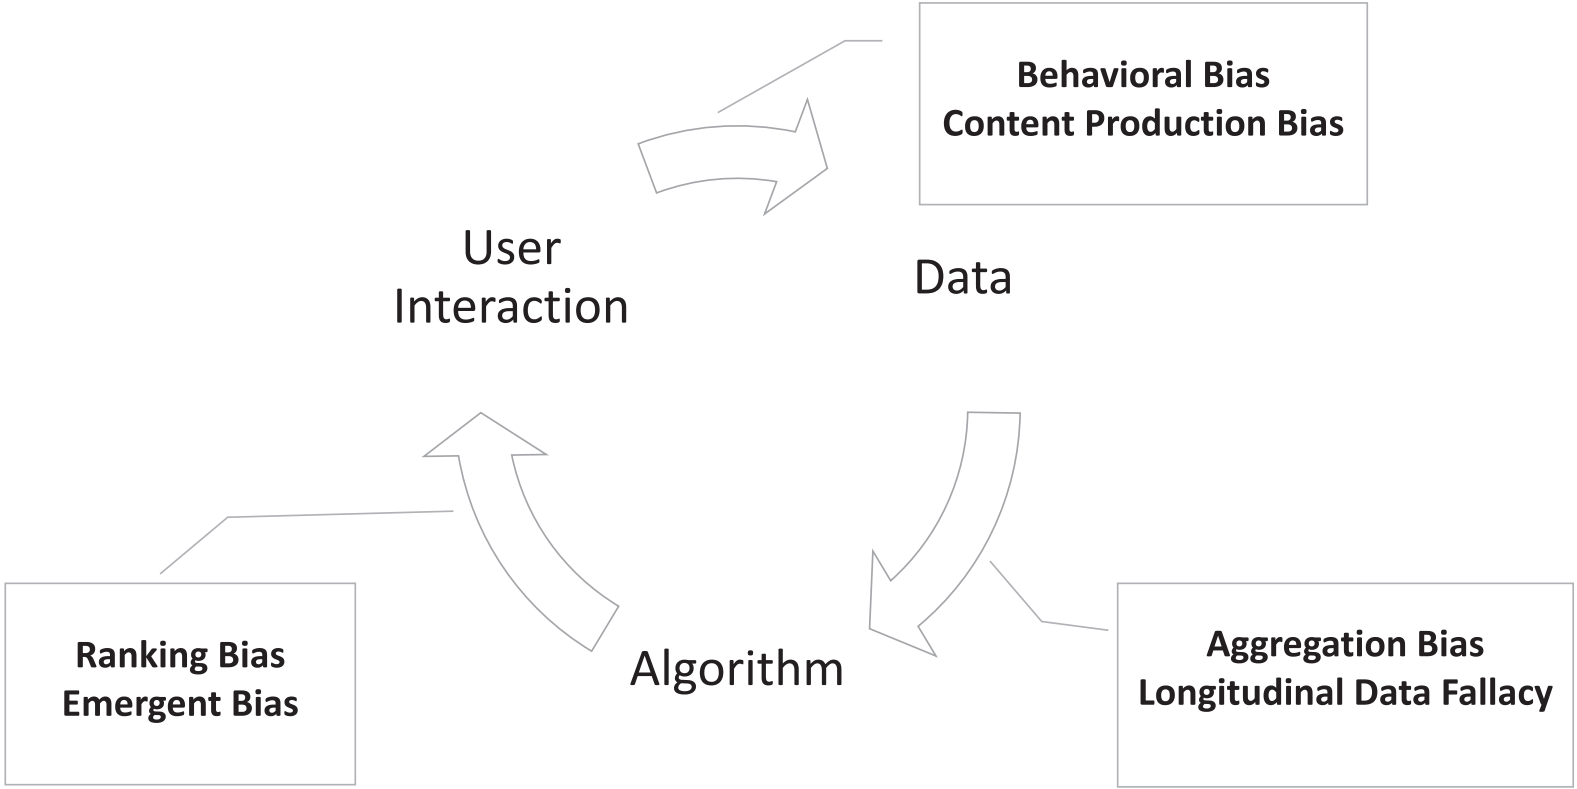
\includegraphics[width=0.8\textwidth]{figures/BiasCategoriesInMLLifecycle.png}
				\caption{Bias definitions in a ML lifecycle \autocite{Mehrabi_2021}.}
				\label{fig:bias_definitions_ML_lifecycle}
			\end{figure}
			
			\rawcitationusedstart
			\begin{itemize}
				\item two potential sources of unfairness in machine learning outcomes - those that arise from biases in the data and those that arise from the algorithms ... we observe that biased algorithmic outcomes might impact user experience, thus generating a feedback loop between data, algorithms and users that can perpetuate and even amplify existing sources of bias \autocite{Mehrabi_2021}.
				\item The loop capturing this feedback between biases in data, algorithms, and user interaction is illustrated in Figure 1. We use this loop to categorize definitions of bias in the section below \autocite{Mehrabi_2021}
			\end{itemize}
			\rawcitationusedend
			
			
			\subsection{Bias Types}
			 The \autoref{tab:biases_types} aims to provide an overview over what kind of biases exist according to research. The more detailed categories listed in the table try to capture similar kind of biases. This thesis follows roughly the categorization of \cite{Mehrabi_2021}. Some biases might acctually fit in multiple categories. The definition of the categories including examples of specific biases follows.
			
			\todo{check categorization of table ref18, statistical biases}
			\todo{check the c citations pls}
			\begin{table}[H]
				\centering
				\begin{threeparttable}
					\begin{tabularx}{\textwidth}{>{\tblWidthDescription}X|>{\tblWidthContext}X|>{\tblWidthContext}X}
						\toprule
						\textbf{Bias} & \multicolumn{2}{c}{\textbf{Mentioned in Context of}} \\
						& \textbf{ML} & \textbf{Dermatology} \\
						%	\midrule
						\multicolumn{3}{l}{\textbf{Data Biases}} \\ 
						\multicolumn{3}{l}{\bolditalic{Sampling Biases}} \\
						Sampling Bias        & X\tnote{1} &    \\
						(Systematic) Selection Bias		 & X\tnote{18} & X\tnote{19,c5,c6,c33,20} \\
						Survivorship Bias    & X\tnote{18} & \\
						Ascertainment Bias	 & X\tnote{16} & X\tnote{19,c9,c10}\\
						
						Healthy Volunteer Selection Bias & X\tnote{14} & \\
						Recall Bias			 & X\tnote{18}& X\tnote{19, c3–c6}\\
						
						\multicolumn{3}{l}{\bolditalic{Demographic and Representation Biases}} \\
						Representation Bias  & X\tnote{1,2,15,20} & X\tnote{21} \\
						Aggregation Bias     & X\tnote{1,2} &   \\
						Omitted Variable Bias & X\tnote{1,11,13,18} &  \\
						
						\multicolumn{3}{l}{\bolditalic{Data Processing and Measurement Biases}} \\
						Measurement Bias     & X\tnote{1,2} &   \\
						Linking Bias         & X\tnote{1,3} &    \\
						Image Quality/Visual Artifacts Bias    & &  X\tnote{20,\todo{add those from young}} \\
						Annotator Bias & & X\tnote{21} \\
						Data dredging bias   & & X\tnote{19,c16-c19} \\
						
						\bolditalic{Temporal Data Biases} & X\tnote{1} & X\tnote{19}\\
						
						\multicolumn{3}{l}{\bolditalic{Clinical and Diagnostic Biases}} \\
						Berkesonian Bias     &            & X\tnote{19,c7}  \\
						Collider Bias        &            & X\tnote{19,c8,c9} \\
						Diagnostic Access Bias & & X\tnote{19,c19,c20,20} \\
						Diagnostic Reference Test Bias & & X\tnote{19,c21} \\
						
						\multicolumn{3}{l}{\bolditalic{Funding and Research Biases}} \\
						Funding / (Industry) Sponsorship Bias    & X\tnote{18} & X\tnote{19} \\
						Hot stuff bias & & X\tnote{19,c22,c23} \\
						Hypothetical Bias    & & X\tnote{19,c31} \\
						Observer Bias		 & X\tnote{18}& X\tnote{19,c29} \\
						
						\multicolumn{3}{l}{\bolditalic{Availability and Selection Biases}} \\
						Availability bias    &  & X\tnote{19,c9} \\
						Informed presence bias & & X\tnote{19,c27} \\
						Mimicry Bias & & X\tnote{19,c28} \\
						Unacceptable Disease Bias & & X\tnote{19,30} \\
						
						%	\midrule
						\multicolumn{3}{l}{\textbf{Algorithmic Biases}} \\ 
						\multicolumn{3}{l}{\bolditalic{Biases in Model Training and Learning}} \\
						Algorithmic Bias     & X\tnote{1,4,5} &   \\
						Emergent Bias        & X\tnote{1,9} &    \\
						Evaluation Bias      & X\tnote{1,2,12} &   \\
						Generalization Issues &  & X\tnote{20,\todo{add those from young}} \\
						
						\multicolumn{3}{l}{\bolditalic{Biases in Predictions and User Interaction}} \\
						User Interaction Bias& X\tnote{1,4} &    \\
						Presentation Bias    & X\tnote{1,4} &    \\
						Ranking Bias         & X\tnote{1,4,6} &    \\
						Popularity Bias      & X\tnote{1,10} & X\tnote{19,c9}   \\
						Incorporation Bias   & & X\tnote{19,c25,c26} \\
						
						%	\midrule
						\multicolumn{3}{l}{\textbf{User Biases}} \\ 
						\multicolumn{3}{l}{\bolditalic{Cognitive and Decision-Making Biases}} \\
						Cognitive Bias    & X\tnote{18} & \\
						Previous opinion Bias & & X\tnote{19, c32} \\
						Confirmation bias &   &X\tnote{19,c15} \\
						Cause-Effect Bias    & X\tnote{18} & \\
						
						\multicolumn{3}{l}{\bolditalic{Behavioral and Social Biases}} \\
						Self-Selection Bias  & X\tnote{1,18,20} &   \\
						Social Bias          & X\tnote{1,4,7} &     \\
						Historical Bias      & X\tnote{1,2,17} &  \\
						Behavioral Bias      & X\tnote{1,3} &    \\
						Temporal Bias        & X\tnote{1,3} &    \\
						
						\multicolumn{3}{l}{\bolditalic{Medical and Publication Biases}} \\
						Content Production Bias & X\tnote{1,3} &    \\
						Publication/All is Well Bias     & \todo{add citation} & X\tnote{19,c10-c12} \\
						Non-Responder bias / Attrition bias      &  & X\tnote{19, c9} \\
						
						\multicolumn{3}{l}{\bolditalic{Population and Perception Biases}} \\
						Population Bias      & X\tnote{1,3,8} &   \\
						
						\multicolumn{3}{l}{\bolditalic{Other Biases}} \\
						Apprehension bias   &  & X\tnote{19,c13} \\
						Rethoric bias & & X\tnote{19, c14} \\
						Centripetal bias &  &X\tnote{19} \\
						Novelty bias & & X\tnote{19} \\
						Language Bias & & X\tnote{19} \\
						
						\bottomrule
					\end{tabularx}
					\begin{tablenotes}
						\footnotesize
						\begin{minipage}{0.33\textwidth}\raggedright
							\item[1] \autocite{Mehrabi_2021}
							\item[2] \autocite{M144_Suresh_2021}
							\item[3] \autocite{M120_Olteanu_2019}
							\item[4] \autocite{M9_Baeza-Yates_2018}
							\item[5] \autocite{M44_Danks_2017}
						\end{minipage}%
						\begin{minipage}{0.33\textwidth}\raggedright
							\item[6] \autocite{M93_Lerman_2014} 
							\item[7] \autocite{M151_Wang_2014} 
							\item[8] \autocite{M64_Hargittai_2007}
							\item[9] \autocite{M53_Friedman_1996}
							\item[10] \autocite{M117_Ciampaglia_2018}
						\end{minipage}%
						\begin{minipage}{0.33\textwidth}\raggedright
							\item[11] \autocites{M38_Clarke_2005}{M131_Riegg_2008}
							\item[12] \autocite{M24_Buolamwini_2018}
							\item[13] \autocite{M114_Mustard_2003}
							\item[14] \autocite{M54_}
							\item[15] \autocite{M142_}
							\item[16] \autocite{M98_}
							\item[17] \autocite{M150_}
							\item[18] \autocites{Mester_2022}{Mester_2017}
							\item[19] \autocite{Chakraborty_2024}
							\item[20] \autocite{Young_2020}
							\item[21] \autocite{Montoya_2025}
						\end{minipage}%
					\end{tablenotes}
				\end{threeparttable}
				\caption{Biases - Mentioned in Contextual Research, grouped like in \cite{Mehrabi_2021}, the author cannot guarantee for completeness}
				\label{tab:biases_types}
			\end{table}
			
			\subsubsection{Data Biases}
				
				\paragraph{Sampling Biases \autocite{Mehrabi_2021} \autocite{Chakraborty_2024}}		
				When gathering data, it's usually not possible to gather the data of a whole population. Instead, the data is gathered by sampling. A sample is a subgroup of individuals from the population. To get unbiased results, this sampling process should represent the true population, with a low sampling error \autocites{HP_2022}. This is often achieved with randomized samples. With non-random sampling processes, sampling bias arises. The consequence is, that the insights of one sampled population may not generalize with insights on another sampled popluation \autocite{Mehrabi_2021}.
				
				Those biases can be introduced with a flawed sampling process:
				\begin{itemize}
					\item \textbf{Sampling bias}, due to nonrandom sampling of subgroups, leading to poor generalization \autocite{Mehrabi_2021}
					\item \textbf{Selection bias}, working only on specific subset of the population which is not representative \autocites{Mestner_2022}{Chakraborty_2024}
					\item \textbf{Systematic selection bias}, chosen samples differ dramatically from the representative populations; e.g. in dermatology, when only the most severe patient data gets included \autocite{Chakraborty_2024, c5,c6,c33}
					\item \textbf{Ascertainment bias}, tendency to exclude segments from the population due to e.g. cultural differences, such as which patient segment goes to government clinics vs. private clinics (usually influenced by socioeconomic status) \autocite{Chakraborty_2024, c5}
					\item \textbf{Availability bias}, focus on widely available data instead of most representative data \autocites{Chakraborty_2024, c9, c10}{}
					\item \textbf{Survivorship bias}, focus only on pre-selected data, ignoring the initial data-points which got filtered out \autocite{Mestner_2022}.
					
					\item \textbf{bias}, what is it, consequence \autocite{}
				\end{itemize}
				
				
				\subparagraph{Potential Biases in PASSION}
				PASSION tries to reduce sampling bias in dermatology against high pigmented skin.
				PASSION might introduce (systematic) selection bias or Ascertainment bias, if in the dermatology centers only sickest / more severe patients are seen as indicated by \cite{Chakraborty_2024}
				PASSION inherits availability bias as it is using \gls{FST} scale.
				Survivorship bias could be relevant for PASSION, if dermatology diseases could be lethal. Further, all patients which are not able to go to one of the dermatology centers which were used in PASSION could be considered to left out by survivorship bias.
				
				\rawcitationstart
				used
				\begin{itemize}		
			 	\rawcitationusedstart
					\item Sampling Bias. Sampling bias is similar to representation bias, and it arises due to nonrandom sampling of subgroups. As a consequence of sampling bias, the trends estimated for one population may not generalize to data collected from a new population. \autocite{Mehrabi_2021}. This is what the PASSION dataset tries to improve
					
					\item Selection bias - wrong sampling method, working on a specific subset of audience; usually by working only with data that is easy to access \autocites{Mester_2022}{Mester_2017} - statistical bias
					\item Selection bias: Since it is not possible to work with large populations, for most dermatological studies, samples are chosen that are said to be representative of the original population. 
					In selection bias, the selected subgroups are not representative of their original population.
					A variation of this is systematic selection bias, where samples chosen differ dramatically from their representative populations.
					Our experience suggests, such selection bias occurs more commonly in studies conducted in regional referral centers where only the sickest or more severe patients are usually seen.
					For example, a study compared the efficacy of thalidomide vs. prednisolone in hospitalised patients of erythema nodosum leprosum. It derived that thalidomide was more efficacious than steroids in erythema nodosum leprosum. Such findings cannot be generalised to all erythema nodosum leprosum since patients admitted to a regional referral center will likely have more severe disease.5,6,33 \autocite{Chakraborty_2024}
					\item  Availability bias: More emphasis is placed on widely available data than scantily available data. A classic example is the use of antihistamines in pregnancy dermatoses, where nearly all standard books recommend first-generation antihistamine chlorpheniramine because more data is available.9 10. \autocite{Chakraborty_2023} - dermatology
					
					\item Survivorship bias \autocites{Mester_2022}{Mester_2017} - statistical bias
					
					
					\item Ascertainment Bias: This bias is commonly encountered in venereology practice. It is defined as a bias due to the tendency of some segments of the target population to get excluded due to cultural and other differences. For example, in most venereology clinics in government setups, studies show that venereal diseases are commoner in lower socioeconomic status. One reason might be that the higher socioeconomic status people tend to go to private practitioners and thereby get excluded from government-run clinics.9,10 Allocation concealment and blinding are good ways to avoid this. 5. \autocite{Chakraborty_2023} - healthcare
				\rawcitationusedend
				\end{itemize}
				
				even more extensive
				\begin{itemize}
					\item Selection bias is again divided into two types endogenous selection bias and exogenous selection bias. The best example of endogenous selection bias in dermatology is the inclusion of non-response. If a trial tests the efficacy of a particular biologic in psoriasis, the response is usually collected from trial participants via postal services. Certain participants will not respond, although they might have substantially improved. Their exclusion will result in significant differences in efficacy evaluation.33
					Exogenous selection bias results when both treatment and outcome result from dependency on an external variable that is not controlled. For example, if sunlight exposure is not controlled, it will influence both the intervention and control groups since psoriasis is a photosensitive (and photoexcerbated) dermatosis. \autocite{Chakraborty_2023} - dermatology
					
					
					\item survivorship bias - World War II planes \autocite{Silfwer_2017} - https://doctorspin.org/media-psychology/psychology/survivorship-bias/
				\end{itemize}
					
				\rawcitationend
					
				\paragraph{Representation Bias \autocite{Mehrabi_2021} \autocite{Chakraborty_2024}}
				\todo{still figure out whether this is a single category, and whether some of the more relevant selection biases should be considered here} 
				
				Those biases can be introduced :
				\begin{itemize}
					\item \textbf{Representation bias}, non-representative sample lead to missing subgroups or other representation anomalies, which can be harmful to downstream applications. Popular ML datasets suffer from representation bias \autocites{Mehrabi_2021}{M142_}
					\item \textbf{Aggregation bias}, what is it, consequence \autocite{}
					\item \textbf{bias}, what is it, consequence \autocite{}
					\item \textbf{bias}, what is it, consequence \autocite{}
				\end{itemize}
				
				
				\subparagraph{Potential Biases in PASSION}
				PASSION tries to mitigate representation bias, by including more FST skin types - however, it could introuce other representation biases
				
				
				\rawcitationstart
				used
				\begin{itemize}		
					\rawcitationusedstart
					\item Representation Bias. Representation bias arises from how we sample from a population during data collection process \autocite{M144_Suresh_2021}. Non-representative samples lack the diversity of the population, with missing subgroups and other anomalies \autocite{Mehrabi_2021}.
					\item Popular machine-learning datasets that serve as a base for most of the developed algorithms and tools can also be biased—which can be harmful to the downstream applications that are based on these datasets. ... In [142], researchers showed that these datasets suffer from representation bias and advocate for the need to incorporate geographic diversity and inclusion while creating such datasets. \autocite{Mehrabi_2021}
					\rawcitationusedend
				\end{itemize}
				
				even more extensive
				\begin{itemize}
					\item 
				\end{itemize}
								
				not checked yet
				\begin{itemize}
					\item Aggregation Bias. Aggregation bias (or ecological fallacy) arises when false conclusions are drawn about individuals from observing the entire population. An example of this type of bias can be seen in clinical aid tools. Consider diabetes patients who have apparent morbidity differences across ethnicities and genders. Specifically, HbA1c levels, that are widely used to diagnose and monitor diabetes, differ in complex ways across genders and ethnicities. Therefore, a model that ignores individual differences will likely not be well-suited for all ethnic and gender groups in the population \autocite{M144_Suresh_2021}. This is true even when they are represented equally in the training data. Any general assumptions about subgroups within the population can result in aggregation bias. \autocite{Mehrabi_2021}. --> could also be important for dermatology issues!!!
					\begin{itemize}
						\item Simpson’s Paradox. Simpson’s paradox is a type of aggregation bias that arises in the analysis of heterogeneous data [18]. The paradox arises when an association observed in aggregated data disappears or reverses when the same data is disaggregated into its underlying subgroups (Fig. 2(a)). ... After analyzing graduate school admissions data, it seemed like there was bias toward women, a smaller fraction of whom were being admitted to graduate programs compared to their male counterparts. However, when admissions data was separated and analyzed over the departments, women applicants had equality and in some cases even a small advantage over men. The paradox happened as women tended to apply to departments with lower admission rates for both genders. Simpson’s paradox has been observed in a variety of domains, including biology [37], psychology [81], astronomy [109], and computational social science [91].\autocite{Mehrabi_2021}.	
						\item Modifiable Areal Unit Problem is a statistical bias in geospatial analysis, which arises when modeling data at different levels of spatial aggregation [56]. This bias results in different trends learned when data is aggregated at different spatial scales \autocite{Mehrabi_2021}.
					\end{itemize}
					
					\item Omitted Variable Bias. Omitted variable bias4 occurs when one or more important variables are left out of the model \autocites{M38_Clarke_2005}{M131_Riegg_2008}\autocite{M114_Mustard_2003}. Something that the model was not ready for\autocite{Mehrabi_2021}. did not take into account
					\item Omitted variable bias \autocites{Mester_2022}{Mester_2017} - statistical bias
				\end{itemize}
				%\rawcitationusedend
				\rawcitationend
			
			\paragraph{Temporal Data Bias}
			Certain studies require to track temporal data, to learn about behaviour or disease progression over time \autocite{Mehrabi_2021}. For PASSION, temporal biases are currently irrelevant, since PASSION contains images independently of time and is not tracking the disease progression. Therefore, the listed biases in this chapter are not explained in detail, refer to the sources for further information.
			
			Examples for temporal data biases are:
			\begin{itemize}
				\item \textbf{Longitudinal Data Fallacy} \autocite{Mehrabi_2021}
				\item \textbf{Chronological bias} \autocite{Chakraborty_2024, c9, c13}
				\item \textbf{Immortal time bias} \autocite{Chakraborty_2024, c24, c20}
			\end{itemize}
			
			
			
			\paragraph{Clinical and Diagnostic Bias \autocite{Chakraborty_2024}}
			In ML for health care, clinical and diagnostic biases require special attention, since they directly influence the diagnosis of a disease.
			\todo{describe difference between clinical and diagnostic, eventually split them}
			
			Those biases can be introduced :
			\begin{itemize}
				\item \textbf{Berkesonian bias} occurs in hospital-based studies when two variables influence hospital or clinical attendance independently. This can lead to a distorted estimation of the relationship between those variables because the study population of hospitalized patients is not representative of the whole population \autocite{Chakraborty_2023, c3, c7}
				\item \textbf{Diagnostic access bias}, depending on the geographical location, individuals have better access to medical care. Therefore, their disease prevalence could appear to be higher and diseases could be diagnosed earlier. \autocite{Chakraborty_2024}
				\item \textbf{Diagnostic reference test bias} is a \textbf{verification bias}, where not all individuals receive the same reference test for the diagnostic process, potentially leading to different diagnoses. \autocite{Chakraborty_2024, c21}
			\end{itemize}
			
			\subparagraph{Potential Biases in PASSION}
			Berkesonian bias depending on the chosen hospitals
			Diagnostic access bias can somewhat be addressed by PASSION, since its dataset includes samples of later states of diseases. However, in the PASSION context itself, this bias could still be relevant.
			Diagnostic reference test bias could be inherited in the PASSION dataset, depending on how the dermatologists work.
			
			
			
			\rawcitationstart
			used
			\begin{itemize}		
				\rawcitationusedstart
					\item Berkesonian Bias: Named after Dr. Joseph Berkeson, this bias reflects the variation in rates of hospital admission or clinic attendance for different diseases. For example, if a study is conducted to know the effect of pregnancy on syphilis in an antenatal clinic, we are likely to get biased data since the two conditions, viz pregnancy and syphilis, are both likely to affect clinic attendance and all observations related to the relationship between pregnancy and syphilis.7 3. \autocite{Chakraborty_2023} - dermatology
					\item  Diagnostic Access Bias: Individuals in certain geographical localities have better access to medical care and, hence, may appear to have higher disease prevalence. For example, atopic dermatitis is believed to be commoner in the West – this could be due to better and earlier diagnostic facilities available than in India.19,20 17.\autocite{Chakraborty_2023}
					\item  Diagnostic reference test bias: These bias results when all individuals do not receive the same reference test. e.g., direct immunofluorescence studies may not be done for all patients with pemphigus vulgaris some patients may receive only a skin biopsy-based diagnosis. It is a subtype of verification bias. Another variation of this type of bias is partial reference bias, where only some of the study participants receive the index and the reference tests.21\autocite{Chakraborty_2023}
				\rawcitationusedend
			\end{itemize}
			
			even more extensive
			\begin{itemize}
				\item 
			\end{itemize}
			\rawcitationend
			
			
			\paragraph{Measurement and Reporting Bias \autocite{Mehrabi_2021} \autocite{Chakraborty_2024}}
			How features are chosen, used, measured and reported can lead to biases \autocites{Mehrabi_2021}{M144_Suresh_2021}.  
			
			Examples for such biases are:
			\begin{itemize}
				\item \textbf{Measurement bias} in general, e.g. using mismeasured \glspl{proxyVar} lead to misinterpretations of the outcome \autocite{Mehrabi_2021}
				\item \textbf{Annotator bias}, what is it, consequence \autocite{}
			\end{itemize}
			
			
			\subparagraph{Potential Biases in PASSION}
			Country of Origin in PASSION depending on the interpretation - should not be used for ethnicity, as this is not linked directly to the genes, see example https://medium.com/bcggamma/practice-ai-responsibly-with-proxy-variable-detection-42c2156ad986
			
			
			\rawcitationstart
			used
			\begin{itemize}		
				\rawcitationusedstart
				\item Measurement Bias. Measurement, or reporting, bias arises from how we choose, utilize, and measure particular features \autocite{M144_Suresh_2021} (e.g. mismeasured proxy variables) \autocite{Mehrabi_2021}. (= e.g. someone who lives at that postal code probably has this ethnicity ); --> could that be an issue with the country of origin feature?
				\item This study found that while using skin tone instead of race for fairness evaluations in computer vision seems objective, the annotation process remains biased by human annotators. Untested scales, unclear procedures, and a lack of awareness about annotator backgrounds and social context significantly influence skin tone labeling. This study exposes how even minor design choices in the annotation process, like scale order (dark to light instead of light to dark) or image context (face or no face, skin lesion presence), can sway agreement and introduce uncertainty in skin tone assessments. ... The researchers emphasize the need for greater transparency, standardized procedures, and careful consideration of annotator biases to mitigate these challenges and ensure fairer and more robust evaluations in computer vision. \autocite{Montoya_2025} - demographic dermatology bias
				
				Quality bias
				\item Image quality. Several barriers to AI implementation in the clinic need to be overcome with regards to imaging (Figure 1). These include technical variations (e.g., camera hardware and software) and differences in image acquisition and quality (e.g., zoom level, focus, lighting, and presence of hair). For example, the presence of surgical ink markings is associated with decreased specificity (Winkler et al., 2019), field of view can significantly affect prediction quality (Mishra et al., 2019), and classification performance improves when hair and rulers are removed (Bisla et al., 2019). We have developed a method to measure how model predictions might be biased by the presence of a visual artifact (e.g., ink) and proposed methods to reduce such biases (Pfau et al., 2019). Poor quality images are often excluded from studies, but the problem of what makes an image adequate is not well studied. Ideally, models need to be able to express a level of confidence in a prediction as a function of image quality and appropriately direct a user to retake photos if needed. \autocite{Young_2020} - dermatology
				
				Reporting bias
				\item  Data dredging bias: It is an entirely avoidable bias. This is subdivided into two types – Fishing type and “P-value hacking” type. It involves using multiple statistical methods to get the desired p-value and selecting the statistical model that gives the p-value the author wants. This is “lamentably common” in dermatological research.16 To detect data dredging bias, always perform a “p-curve analysis” while performing a meta-analysis.17,18 Much emphasis is nowadays given to the confidence interval instead of the p-value, which gives an approximate idea of the range in which one can be 95\% (or 90\%, depending on the confidence interval chosen) sure that the result is correct. The confidence interval remains unaffected by p-value dredging. This subject has been reviewed in depth in recent works.18,19 15.\autocite{Chakraborty_2023}
				\rawcitationusedend
			\end{itemize}
			
			even more extensive
			\begin{itemize}
				\item 
			\end{itemize}
			
			not checked yet
			\begin{itemize}
				\item 
			\end{itemize}
			\rawcitationend
			
			\rawcitationstart
			others
			\begin{itemize}
				\item \todo{check if healthy volunteer is self-selection bias} Other such studies were conducted in [54] which states that UK Biobank, a large and widely used genetic dataset, may not represent the sampling population. Researchers found evidence of a “healthy volunteer” selection bias. [150] has other examples of studies on existing biases in the data used in the medical domain. [157] also looks at machine-learning algorithms and data utilized in medical fields, and writes about how artificial intelligence in health care has not impacted all patients equally.\autocite{Mehrabi_2021} --> [150] also provides an ovverview over the impact of social determinants on health, such as Economic stability, neighborhood and physical environment, education, food, community and scial context, access to healthcare and quality
				\item Recall bias - respondent doesn't remember things correctly; Recall bias is another common error of interview/survey situations. It happens when the respondent doesn’t remember things correctly. It’s not about bad or good memory – humans have selective memory by default. After a few years (or even a few days), certain things stay and others fade. It’s normal, but it makes research much more difficult. \todo{keep an eye on this when recalling evidences!!}
				
				\autocites{Mester_2022}{Mester_2017} - statistical bias
				\item Memory or recall bias: This is a type of bias where sufferers of a disease, often termed cases, have a greater tendency to recall a particular habit than non-sufferers, viz controls. This results in an uneven distribution of risk factors between the cases and controls. An example of this would be a case-control study to evaluate the association between dental amalgam use and the development of oral lichen planus. Those with lichen planus are more likely to recall a history of dental amalgam use than those who do not have the disease. This difference in recall between a diseased cohort and control has resulted in difficulties in assessing the association between diet and many dermatological diseases – like milk and chocolate consumption and acne, fatty meals and psoriasis, sugary meals and psoriasis, agricultural exposure to insecticides and pemphigus and so on.3–6 2. \autocite{Chakraborty_2023} - dermatology
				\item Collider Bias: This is an under-appreciated bias, and often confused with a confounder. This is especially seen in observational studies where it is defined as a distortion produced by the restriction of sampling by a collider variable. A collider variable is defined as one that has an independent effect on the outcome studied apart from the studied variable. In simpler terms, collider bias occurs when exposure and development influence a common third variable. That variable or collider is controlled by study design or in the analysis. An example is the observation that psoriasis patients tend to have more depression and anxiety disorders. Since severe psoriasis patients tend to get hospitalised and also get screened for mental health issues, a spurious association between them could have been obtained due to collider bias. The two variables viz psoriasis and depression converged, i.e., collided, into a single outcome – hospitalization.8,9 4. \autocite{Chakraborty_2023} - dermatology
				
				\item Linking Bias. Linking bias arises when network attributes obtained from user connections, activities, or interactions differ and misrepresent the true behavior of the users \autocite{M120_Olteanu_2019} \autocite{Mehrabi_2021}. --> probably less important since we got individuals? Or could that be an issue with the country of origin feature?
			\end{itemize}
			\rawcitationend
			
			\paragraph{ Bias \autocite{Mehrabi_2021} \autocite{Chakraborty_2024}}
			
			Those biases can be introduced :
			\begin{itemize}
				\item \textbf{bias}, what is it, consequence \autocite{}
				\item \textbf{bias}, what is it, consequence \autocite{}
				\item \textbf{bias}, what is it, consequence \autocite{}
				\item \textbf{bias}, what is it, consequence \autocite{}
			\end{itemize}
			
			
			\subparagraph{Potential Biases in PASSION}
			
			\rawcitationstart
			used
			\begin{itemize}		
				\rawcitationusedstart
				\item 
				\rawcitationusedend
			\end{itemize}
			
			even more extensive
			\begin{itemize}
				\item 
			\end{itemize}
			
			not checked yet
			\begin{itemize}
				\item 
			\end{itemize}
			\rawcitationend
			
			
			\subsection{Sensitive Features}
			Research showed sensitive features which are prone to bias. Those led to issues in existing AI applications and their usage should therefore be investigated carefully.
			
			\ref{tab:biases_features} summarizes mentioned features. Since PASSION tries to improve the classification of skin diseases with photographs alone, those features which directly influence the appearance of a disease on the skin are most important. Skin type including undertone are affecting the diseases appearance, but also genetic factors, gender and the age \todo{doublecheck impact of age} of a patient can influence how the diseases manifest themselves. Therefore, they are directly relevant for skin detection and must be considered in the dataset.
			
			Other demographic factors can have an impact on the progression of skin diseases or increase the prevalence of skin conditions (e.g. tropical vs dry climates) \todo{add source}. While this information could support the diagnostic process, it is not visible in the images. Therefore, they could potentially be relevant and enhance the diagnostic process when included into the PASSION dataset. However, the linkage is weak and could introduce further biases.
			
			For completeness, \ref{tab:biases_features} shows further sensitive demographic features which seem not to be linked to dermatology according to research.
			
			
			\todo{check what to do with those additional features:}
			Other important features according to (\autocite{Montoya_2025} 13):
			lesion type, anatomical location of lesion, img characteristics such as source, imaging techniques, resolution, real vs. artificially generated
			\begin{table}[H]
				\centering
				\begin{threeparttable}
					\begin{tabularx}{\textwidth}{>{\tblWidthDescription}X|>{\tblWidthContext}X|>{\tblWidthContext}X}
						\toprule
						\textbf{Bias sensitive Features} & \multicolumn{2}{c}{\textbf{Mentioned in Context of}} \\
						& \textbf{ML} & \textbf{Dermatology} \\
						%\midrule
						\multicolumn{3}{l}{\bolditalic{Dermatology Related Features}} \\
						Skin Type & X\tnote{1,2,7,12} & X\tnote{2,13}\\
						Skin Undertones & & X\tnote{13} \\
						
						\multicolumn{3}{l}{\bolditalic{Demographic Features with Direct Relevance for Skin Disease Detection}} \\
						Age & X\tnote{7,11} &  X\tnote{13} \\
						Ethnicity/Race \todo{check definitions} & X\tnote{1,2,4,5,6,7,11,12}&  X\tnote{13} \\
						Gender/Sex & X\tnote{1,2,7,8,9,10,11} & X\tnote{13} \\
						Gender and Skin Type Subgroups & X\tnote{1,2} & \\
						
						\multicolumn{3}{l}{\bolditalic{Demographic Features Potential Relevance for Skin Disease Detection}} \\
						Geographic Location & X\tnote{1,3} & \\
						Socio-Economic Status & X\tnote{6,12} & \\
						Disabilities & X\tnote{7,11} & \\
						
						\multicolumn{3}{l}{\bolditalic{Demographic Features no Relevance for Skin Disease Detection}} \\
						Familial status & X\tnote{7} & \\
						Marital status & X\tnote{7,11} & \\
						Nationality/National origin & X\tnote{7,11} & \\
						Recipient of public assistance & X\tnote{7} & \\
						Religion & X\tnote{7,11} & \\
						\bottomrule
					\end{tabularx}
					\begin{tablenotes}
						\footnotesize
						\begin{minipage}{0.33\textwidth}\raggedright
							\item[1] \autocite{Mehrabi_2021}
							\item[2] \autocite{M24_Buolamwini_2018}
							\item[3] \autocite{M142_}
							\item[4] \autocite{M98_}
						\end{minipage}%
						\begin{minipage}{0.33\textwidth}\raggedright
							\item[5] \autocite{M54_}
							\item[6] \autocite{M150_}
							\item[7] \autocite{M30_}
							\item[8] \autocite{M167_}
						\end{minipage}%
						\begin{minipage}{0.33\textwidth}\raggedright
							\item[9] \autocite{M20_}
							\item[10] \autocite{M168_}
							\item[11] \autocite{M62_}
							\item[12] \autocite{Young_2020}
							\item[13] \autocite{Montoya_2025}
						\end{minipage}%
					\end{tablenotes}
				\end{threeparttable}
				\caption{Features which often hold biases - Mentioned in Contextual Research, grouped like in \cite{Mehrabi_2021}, the author cannot guarantee for completeness}
				\label{tab:biases_features}
			\end{table}
			
			
		\section{Fairness}
			
			
			
		\section{Mitigation Methods}
			
			
			
		\section{Extensive Sources}
			
			\rawcitationstart
			\subsection{Discrimination vs. Biases}
			\begin{itemize}
				\item bias and discrimination = source of unfairness. Discrimination can be considered as a source for unfairness that is due to human prejudice and stereotyping based on the sensitive attributes, which may happen intentionally or unintentionally, while bias can be considered as a source for unfairness that is due to the data collection, sampling, and measurement. Although bias can also be seen as a source of unfairness that is due to human prejudice and stereotyping, in the algorithmic fairness literature it is more intuitive to categorize them as such according to the existing research in these areas. In this survey, we mainly focus on concepts that are relevant to algorithmic fairness issues. \autocite{Mehrabi_2021}
				\item Explainable Discrimination. Differences in treatment and outcomes amongst different groups can be justified and explained via some attributes in some cases. In situations where these differences are justified and explained, it is not considered to be illegal discrimination and hence called explainable [77]. In [77], authors present a methodology to quantify the explainable and illegal discrimination in data. They argue that methods that do not take the explainable part of the discrimination into account may result in non-desirable outcomes, so they introduce a reverse discrimination which is equally harmful and undesirable. They explain how to quantify and measure discrimination in data or a classifier’s decisions which directly considers illegal and explainable discrimination.\autocite{Mehrabi_2021}
				\item Unexplainable Discrimination. In contrast to explainable discrimination, there is unexplainable discrimination in which the discrimination toward a group is unjustified and therefore considered illegal. Authors in [77] also present local techniques for removing only the illegal or unexplainable discrimination, allowing only for explainable differences in decisions. These are preprocessing techniques that change the training data such that it contains no unexplainable discrimination. We expect classifiers trained on this preprocessed data to not capture illegal or unexplainable discrimination. Unexplainable discrimination consists of direct and indirect discrimination.\autocite{Mehrabi_2021}
				\begin{itemize}
					\item Direct Discrimination. Direct discrimination happens when protected attributes of individuals explicitly result in non-favorable outcomes toward them [164]. ... these traits that are considered to be “protected” or “sensitive” attributes in computer science literature  \autocite{Mehrabi_2021}
					\item Indirect Discrimination. In indirect discrimination, individuals appear to be treated based on seemingly neutral and non-protected attributes; however, protected groups, or individuals still get to be treated unjustly as a result of implicit effects from their protected attributes \autocite{Mehrabi_2021}
				\end{itemize}
				\item Discrimination can be either direct or indirect. Direct discrimination occurs when decisions are made based on sensitive attributes. Indirect discrimination occurs when decisions are made based on nonsensitive attributes which are strongly correlated with biased sensitive ones \autocite{M62_}
				\item ML algorithms reflect cognitive biases in humans, which can result in predictions and decisions that are “unfair” [5]. Unfairness in ML decision-making equates to prejudice or favoritism based on inherent or acquired characteristics of an individual or group [6]. Within medical research, the term bias refers to “a feature of the design of a study, or the execution of a study, or the analysis of the data from a study, that makes evidence misleading” [7,8]. \autocite{Montonaya_2025}
			\end{itemize}
		
		
		\section{General ML biases}
		
			\subsection{Bias Introduction}
			\begin{itemize}
				\item compared SAVRY, a tool used in risk assessment frameworks that includes human intervention in its process, with automatic machine learning methods in order to see which one is more accurate and more fair. Conducting these types of studies should be done more frequently, but prior to releasing the tools in order to avoid doing harm \autocite{Mehrabi_2021}.
				\item \textbf{Assessment Tools} An interesting direction that researchers have taken is introducing tools that can assess the amount of fairness in a tool or system. For example, Aequitas [136] is a toolkit that lets users to test models with regards to several bias and fairness metrics for different population subgroups. Aequitas produces reports from the obtained data that helps data scientists, machine learning researchers, and policymakers to make conscious decisions and avoid harm and damage toward certain populations. AI Fairness 360 (AIF360) is another toolkit developed by IBM in order to help moving fairness research algorithms into an industrial setting and to create a benchmark for fairness algorithms to get evaluated and an environment for fairness researchers to share their ideas [11]. These types of toolkits can be helpful for learners, researchers, and people working in the industry to move towards developing fair machine learning application away from discriminatory behavior \autocite{Mehrabi_2021}.
				\item At first sight, automating decisions may give a sense of fairness: classification rules do not guide themselves by personal preferences. However, at a closer look, one realizes that classification rules are actually learned by the system (e.g., loan granting) from the training data. If the training data are inherently biased for or against a particular community (e.g., foreigners), the learned model may show a discriminatory prejudiced behavior. In other words, the system may infer that just being foreign is a legitimate reason for loan denial. \autocite{M62_}
				\item One might think of a straightforward preprocessing approach consisting of just removing the discriminatory attributes from the data set. Although this would solve the direct discrimination problem, it would cause much information loss and in general it would not solve indirect discrimination. \autocite{M62_}
				\item Hence, there are two important challenges regarding discrimination prevention: one challenge is to consider both direct and indirect discrimination instead of only direct discrimination; the other challenge is to find a good tradeoff between discrimination removal and the quality of the resulting training data sets and data mining models. \autocite{M62_}
			\end{itemize}	
			
			\begin{itemize}
				\item Most AI systems and algorithms are data driven and require data upon which to be trained. Thus, data is tightly coupled to the functionality of these algorithms and systems. In the cases where the underlying training data contains biases, the algorithms trained on them will learn these biases and reflect them into their predictions. As a result, existing biases in data can affect the algorithms using the data, producing biased outcomes. Algorithms can even amplify and perpetuate existing biases in the data.\autocite{Mehrabi_2021}.
				\item In addition, algorithms themselves can display biased behavior due to certain design choices, even if the data itself is not biased. The outcomes of these biased algorithms can then be fed into real-world systems and affect users’ decisions, which will result in more biased data for training future algorithms.\autocite{Mehrabi_2021}.
				
				\item Bias can exist in many shapes and forms, some of which can lead to unfairness in different downstream learning tasks. In \autocite{M144_Suresh_2021}, authors talk about sources of bias in machine learning with their categorizations and descriptions in order to motivate future solutions to each of the sources of bias introduced in the paper. In \autocite{M120_Olteanu_2019}, the authors prepare a complete list of different types of biases with their corresponding definitions that exist in different cycles from data origins to its collection and its processing.\autocite{Mehrabi_2021}.
			\end{itemize}	
			
			\begin{itemize}
				\item The list of biases that can occur in any research is considerably long, and certainly not all of them can be avoided. However, dermatologists should be well aware of them because: 1. While conducting systematic reviews and metaanalysis, PRISMA guidelines need to be followed, and the PRISMA checklist requires a very exhaustive list of declarations to be made by the authors as to how biases in the individual studies were detected, their types and whether they were included in the systematic review or not. This usually requires more than two authors working independently. 2. Biases can result in dramatically opposite inferences, which may not be biologically plausible; the knowledge of the biases can help detect them and thereby negate such findings. 3. The knowledge of biases is a vital part of the postgraduate dermatology curriculum and is a mustknow area for thesis/dissertation purposes. 4. Since there is no fool-proof way to avoid all biases, the help of a well-qualified biostatistician might help detect and prevent many of these biases in research. \autocite{Chakraborty_2024}
			\end{itemize}
			\rawcitationend
			
			Already rewritten: The following categorization was modeled with the intent to show that the different biases are intertwined and one should consider the effects between each other in the cycle to address them correctly \autocite{Mehrabi_2021}
		




			\rawcitationstart
			\subsection{Biases Extensive Sources}
			
			\paragraph{Data Biases}
			Data biases (data to algorithm (biases in data which might have an impact on biased algorithmic outcomes \autocite{Mehrabi_2021}))	
			\begin{itemize}
				\item 
			\end{itemize}	
			
			
			\paragraph{Algorithmic Biases}
			
			Algorithmic biases (Algorithm to user (A modulates U behaviour, biases in algorithm might lead to introduce biases in user behaviour and affect it as a consequence)) \autocite{Mehrabi_2021}
			\begin{itemize}
				\item Algorithmic Bias. Algorithmic bias is when the bias is not present in the input data and is added purely by the algorithm \autocite{M9_Baeza-Yates_2018}. The algorithmic design choices, such as use of certain optimization functions, regularizations, choices in applying regression models on the data as a whole or considering subgroups, and the general use of statistically biased estimators in algorithms \autocite{M44_Danks_2017}, can all contribute to biased algorithmic decisions that can bias the outcome of the algorithms.\autocite{Mehrabi_2021}.
				\item User Interaction Bias. User Interaction bias is a type of bias that can not only be observant on the Web but also get triggered from two sources—the user interface and through the user itself by imposing his/her self-selected biased behavior and interaction \autocite{M9_Baeza-Yates_2018}. This type of bias can be influenced by other types and subtypes, such as presentation and ranking biases. \autocite{Mehrabi_2021}. -- more relevant for later, when the application would become bigger
				\begin{itemize}
					\item Presentation Bias. Presentation bias is a result of how information is presented \autocite{M9_Baeza-Yates_2018} (can only click on content they see, could be the case that user does not see all info on web) \autocite{Mehrabi_2021}.
					\item Ranking Bias. The idea that top-ranked results are the most relevant and important will result in attraction of more clicks than others. This bias affects search engines \autocite{M9_Baeza-Yates_2018} and crowdsourcing applications \autocite{M93_Lerman_2014}.\autocite{Mehrabi_2021}.
				\end{itemize}
				\item Popularity Bias. Items that are more popular tend to be exposed more. However, popularity metrics are subject to manipulation—for example, by fake reviews or social bots \autocite{M117_Ciampaglia_2018}. ... this presentation may not be a result of good quality; instead, it may be due to other biased factors. \autocite{Mehrabi_2021}.
				\item Emergent Bias. Emergent bias occurs as a result of use and interaction with real users. This bias arises as a result of change in population, cultural values, or societal knowledge usually some time after the completion of design \autocite{M53_Friedman_1996}. This type of bias is more likely to be observed in user interfaces, ... This type of bias can itself be divided into more subtypes, as discussed in detail in \autocite{M53_Friedman_1996}. \autocite{Mehrabi_2021}. probably less relevant at the first stage
				\item Evaluation Bias. Evaluation bias happens during model evaluation \autocite{M144_Suresh_2021}. This includes the use of inappropriate and disproportionate benchmarks for evaluation of applications such as Adience and IJB-A benchmarks. These benchmarks are used in the evaluation of facial recognition systems that were biased toward skin color and gender \autocite{M24_Buolamwini_2018}, and can serve as examples for this type of bias \autocite{M144_Suresh_2021}. \autocite{Mehrabi_2021}. -- important for this thesis
			\end{itemize}
			
			\paragraph{User Biases}
			
			User to Data (user-generated data, inherent biases in users could be reflected in the data they generate; biases in last section might introduce further bias in this process) \autocite{Mehrabi_2021}
			\begin{itemize}
				\item Historical Bias. Historical bias is the already existing bias and socio-technical issues in the world and can seep into from the data generation process even given a perfect sampling and feature selection \autocite{M144_Suresh_2021}. ... search results were of course reflecting the reality, but whether or not the search algorithms should reflect this reality is an issue worth considering \autocite{Mehrabi_2021} - maybe relevant
				\item Population Bias. Population bias arises when statistics, demographics, representatives, and user characteristics are different in the user population of the platform from the original target population \autocite{M120_Olteanu_2019}. Population bias creates non-representative data. ... More such examples and statistics related to social media use among young adults according to gender, race, ethnicity, and parental educational background can be found in \autocite{M64_Hargittai_2007}. \autocite{Mehrabi_2021}
				\item Self-Selection Bias. Self-selection bias4 is a subtype of the selection or sampling bias in which subjects of the research select themselves. \autocite{Mehrabi_2021}
				\item Social Bias. Social bias happens when others’ actions affect our judgment \autocite{M9_Baeza-Yates_2018}. (case where we want to rate or review an item with a low score, but when influenced by other high ratings, we change our scoring thinking that perhaps we are being too harsh [\autocite{M9_Baeza-Yates_2018}, \autocite{M151_Wang_2014}.) \autocite{Mehrabi_2021}
				\item Behavioral Bias. Behavioral bias arises from different user behavior across platforms, contexts, or different datasets \autocite{M120_Olteanu_2019}. \autocite{Mehrabi_2021} maybe, people from different countries go to the dermatologist for different diseases, based on cultural differences?
				\item Temporal Bias. Temporal bias arises from differences in populations and behaviors over time \autocite{M120_Olteanu_2019}. \autocite{Mehrabi_2021} -- could this also be differences in the year, when people go to dermatologists? over which timeline has the PASSION data been captured? 
				\item Content Production Bias. Content Production bias arises from structural, lexical, semantic, and syntactic differences in the contents generated by users \autocite{M120_Olteanu_2019}. \autocite{Mehrabi_2021} -- could the quality of the pictures been related to this as well?
			\end{itemize}
		
			\paragraph{Dermatology Biases}
			\begin{itemize}
				\item Equity. AI has the potential to worsen health-care disparities, as recognized by the popular media (Khullar, 2019), particularly in dermatology (Adamson and Smith, 2018). The first concern is adequate representation of underserved populations in training data. Existing DL models have been trained on mainly European or East Asian populations, and the relative lack of training on darker skin pigmentation may limit overall diagnostic accuracy. This possibility is demonstrated by the increased error rates in commercial systems, trained on predominantly white datasets, for facial analysis in identifying black individuals (Buolamwini and Gebru, 2018). Second, AI may entrench existing social and economic biases and perpetuate inadvertent discriminatory practices, for example, in recommending less follow-up for black patients than for whites, when health costs are used as a proxy for health needs (Obermeyer et al., 2019). Third, disproportionate adoption by different groups may exacerbate existing inequities. Access to and use of technology differs based on sociodemographics (Tsetsi and Rains, 2017), and more techsavvy users may be more likely to embrace AI for skin screening (Tong and Sopory, 2019). The issue of equity in AI diagnosis needs to be carefully addressed to avoid inadvertent exacerbation of health-care disparities. \autocite{Young_2020} - dermatology
				\item Model generalizability. Generalizability is a major concern for AI models; studies of computer-assisted diagnosis of melanoma report lower sensitivity for melanoma on independent test sets than on nonindependent test sets (Dick et al., 2019). It is difficult to study generalizability because published DL models are not publicly available, making it impossible to compare performance, unless each study uses a standardized benchmark database, such as the Melanoma Classification Benchmark (Brinker et al., 2019d). Han et al. (2018a) reported excellent metrics of performance and made their model available for image submission; however, the model prediction was not robust when images from an outside clinic were submitted, image magnification or contrast was altered, or images were rotated (NavarreteDechent et al., 2018). On ImageNet, a nonmedical dataset of 1,000 object categories, training on a dataset of 300 ... \autocite{Young_2020}
			\end{itemize}
			\paragraph{Papers I would need access to}
			\begin{itemize}
				\item https://jamanetwork.com/journals/jamadermatology/article-abstract/2688587 (linked to \autocite{Young_2020})
				\item https://academic.oup.com/bjd/article-abstract/190/6/789/7603706?redirectedFrom=fulltext Ethical considerations for artificial intelligence in dermatology: a scoping review
				
			\end{itemize}
			\rawcitationend
			
		    \subsection{Fairness Overview}
			\begin{table}[H]
				\centering
				\begin{threeparttable}
					\begin{tabularx}{\textwidth}{>{\tblWidthDescription}X|>{\tblWidthContext}X|>{\tblWidthContext}X}
						\toprule
						\textbf{Fairness Definitions} & \multicolumn{2}{c}{\textbf{Mentioned in Context of}} \\
						& \textbf{ML} & \textbf{Dermatology} \\
						%	\midrule
						\multicolumn{3}{l}{\textbf{Group Fairness}} \\ 
						Conditional Statistical Parity    & X\tnote{1,3,10} &   \\
						Demographic/Statistical Parity  & X\tnote{1,3,4,5} &   \\
						Equalized Odds     & X\tnote{1,2,3} &   \\
						Equal Opportunity& X\tnote{1,2,3} &   \\
						Treatment Equality & X\tnote{1,7} &   \\
						Test Fairness         & X\tnote{1,3,8} &   \\
						%	\midrule
						\multicolumn{3}{l}{\textbf{Subgroup Fairness}} \\ 
						Subgroup Fairness    & X\tnote{1,11,12} &   \\
						%\midrule
						\multicolumn{3}{l}{\textbf{Individual Fairness}} \\ 
						Counterfactual Fairness     & X\tnote{1,5} &   \\
						Fairness Through Awareness     & X\tnote{1,4,5} &   \\
						Fairness Through Unawareness        & X\tnote{1,5,6} &   \\
						%\midrule
						\multicolumn{3}{l}{\textbf{Not Categorized}} \\ 
						Fairness in Relational Domains& X\tnote{1,9} &   \\
						\bottomrule
					\end{tabularx}
					\begin{tablenotes}
						\footnotesize
						\begin{minipage}{0.33\textwidth}\raggedright
							\item[1] \autocite{Mehrabi_2021}
							\item[2] \autocite{M63_Hardt_2016}
							\item[3] \autocite{M149_Verma_2018}
							\item[4] \autocite{M48_Dwork_2012}
						\end{minipage}%
						\begin{minipage}{0.33\textwidth}\raggedright
							\item[5] \autocite{M87_Kusner_2017}
							\item[6] \autocite{M61_Grgic-Hlaca_2016}
							\item[7] \autocite{M15_Berk_2017}
							\item[8] \autocite{M34_Chouldechova_2017}
						\end{minipage}%
						\begin{minipage}{0.33\textwidth}\raggedright
							\item[9] \autocite{M50_Farnadi_2018}
							\item[10] \autocite{M41_Corbett-Davies_2017}
							\item[11] \autocite{M79_Kearns_2018}
							\item[12] \autocite{M80_Kearns_2019} \todo{potential bias in this bc same author of the algorithm tested it}
						\end{minipage}%
					\end{tablenotes}
				\end{threeparttable}
				\caption{Fairness Definitions - Mentioned in Contextual Research, grouped like in \cite{Mehrabi_2021}, the author cannot guarantee for completeness}
				\label{tab:fairness_definitions}
			\end{table}
			
			\rawcitationstart
			\subsection{Fairness Extensive Sources}
			\paragraph{Algorithmic Fairness}
			\begin{itemize}
				\item in order to be able to fight against discrimination and achieve fairness, one should first define fairness. \autocite{Mehrabi_2021}
				\item The fact that no universal definition of fairness exists shows the difficulty of solving this problem [138]. Different preferences and outlooks in different cultures lend a preference to different ways of looking at fairness, which makes it harder to come up with just a single definition that is acceptable to everyone in a situation. there is still no clear agreement on which constraints are the most appropriate for those problems. \autocite{Mehrabi_2021}
				\item Broadly, fairness is the absence of any prejudice or favoritism towards an individual or a group based on their intrinsic or acquired traits in the context of decision-making [139]. Even though fairness is an incredibly desirable quality in society, it can be surprisingly difficult to achieve in practice. \autocite{Mehrabi_2021}
				\item Here we will reiterate and provide some of the most widely used definitions, along with their explanations inspired from \autocite{M149_Verma_2018}.\autocite{Mehrabi_2021}
				\item Definitions on page 12, 13, 14 \autocite{Mehrabi_2021}
				\begin{itemize}
					\item Equalized Odds (TP and FP rate should be the same for individuals in different sub groups) \autocite{Mehrabi_2021}
					\item Equal Opportunity (TP rate should be the same) \autocite{Mehrabi_2021}
					\item Demographic Parity / Statistical Parity (likelihood of positive outcome the same regardless of protected group) \autocite{Mehrabi_2021}
					\item Fairness Through Awareness (similar predictions to similar individuals (similarity = inverse distance)) \autocite{Mehrabi_2021}
					\item Fairness Through Unawareness (no protected attributes explicitly used in decision-making process) \autocite{Mehrabi_2021}
					\item Treatment Equality (Ration FN and FP same for both protected group categories) \autocite{Mehrabi_2021}
					\item Test Fairness (for predicted probability scores, people in both groups must have equal probability of TP) \autocite{Mehrabi_2021}
					\item Counterfactual Fairness (same outcome in actual world and counterfactual world where the individual belonged to a different demographic group) \autocite{Mehrabi_2021}
					\item Fairness in Relational Domains (“A notion of fairness that is able to capture the relational structure in a domain—not only by taking attributes of individuals into consideration but by taking into account the social, organizational, and other connections between individuals” \autocite{M50_Farnadi_2018}) \autocite{Mehrabi_2021} probably not relevant since not relational
					\item Conditional Statistical Parity (people in both groups have equal possibilities of being assigned to a positive outcome given a set of legitimate factors) \autocite{Mehrabi_2021}
					\item My text: The survey categorizes those fairness notions in three different groups: Individual Fairness, Group Fairness and Subgroup fairness.  \autocite{Mehrabi_2021}
					\item Subgroup fairness: Subgroup fairness intends to obtain the best properties of the group and individual notions of fairness. It is different than these notions but uses them in order to obtain better outcomes. It picks a group fairness constraint like equalizing false positive and asks whether this constraint holds over a large collection of subgroups \autocite{M79_Kearns_2018}\autocite{M80_Kearns_2019}\autocite{Mehrabi_2021}
					\item it is impossible to satisfy some of the fairness constraints at once except in highly constrained special cases. In [83], the authors show the inherent incompatibility of two conditions: calibration and balancing the positive and negative classes. These cannot be satisfied simultaneously with each other unless under certain constraints; therefore, it is important to take the context and application in which fairness definitions need to be used into consideration and use them accordingly [141]\autocite{Mehrabi_2021}
					\item Another important aspect to consider is time and temporal analysis of the impacts that these definitions may have on individuals or groups. In [95] authors show that current fairness definitions are not always helpful and do not promote improvement for sensitive groups—and can actually be harmful when analyzed over time in some cases. They also show that measurement errors can also act in favor of these fairness definitions; therefore, they show how temporal modeling and measurement are important in evaluation of fairness criteria and introduce a new range of trade-offs and challenges toward this direction. It is also important to pay attention to the sources of bias and their types when trying to solve fairness-related questions. \autocite{Mehrabi_2021}
				\end{itemize}
			\end{itemize}
			\rawcitationend
			
			\subsection{Mitigation Methods Overview}
				\todo{write definitions of pre-in and post-processing, see Methods for fair machine learning below [43, 11, 14]}

				\todo{double check and futher improve groups}
				\begin{table}[H]
				\centering
				\begin{threeparttable}
						\begin{tabularx}{\textwidth}{>{\tblWidthDescription}X|>{\tblWidthContext}X|>{\tblWidthContext}X}
						\toprule
						\textbf{Mitigation Methods - Unbiasing Data (Pre-Processing)} & \multicolumn{2}{c}{\textbf{Mentioned in Context of}} \\
						& \textbf{ML} & \textbf{Dermatology} \\
						\multicolumn{3}{l}{\textbf{Documentation and Transparency}} \\
						Good Practices while using Data & X\tnote{1,2,3} &   \\
						Datasheets as supporting document for dataset creation method, characteristics, motivations and skews & X\tnote{1,2,3} &   \\
						Datasheets as supporting document for model method, characteristics, motivations and skews & X\tnote{1,4} &   \\
						Dataset (Nutrition) Labels & X\tnote{1,5,6} & X\tnote{18, \todo{add spec source}}   \\
						
						\multicolumn{3}{l}{\textbf{Communication and Reporting}} \\
						Messaging & X\tnote{1,12} &   \\
						
						\multicolumn{3}{l}{\textbf{Bias Detection and Evaluation}} \\
						Test for Simpson's Paradox \todo{Discribe Simpson's Paradox} & X\tnote{1,7,8,9} &   \\
						Detect Direct Discrimination with Causal Models and Graphs & X\tnote{1,10} &   \\					
						Out-of-Distribution Detection in Dermatology Using Input Perturbation and Subset Scanning & & X\tnote{19} \\
						Check confidence interval and p-curve analysis instead of p-value & & X\tnote{17} \\
						 
						\multicolumn{3}{l}{\textbf{Study Design}} \\ 
						Allocation concealment and blinding & & X\tnote{17} \\
						Preventing Direct and Indirect Discrimination & X\tnote{1,11} &   \\
						
						\multicolumn{3}{l}{\textbf{Data Gathering}} \\ 
						Data Collection from diverse sources (incl. primary care clinics) & X\tnote{18} & \\
						Robust standards for external validation & X\tnote{18} & \\
						Preferential Sampling & X\tnote{1,13,14} &   \\
						Geographical Diversity and Inclusion for Dataset creation & X\tnote{16} & \\
						Balanced Representation accross skin tones and genders & & X\tnote{19} \\
						Disparate Impact Removal & X\tnote{1,15} &   \\
						
						\multicolumn{3}{l}{\textbf{Labeling}} \\ 
						Multidimensional Scale for Skin Tones & & X\tnote{19} \\
						
						
						\multicolumn{3}{l}{\textbf{Data Availability and Open Science}} \\ 
						Publish Datasets accessible for the public & & X\tnote{18, \todo{add source}} \\						
						
						\bottomrule
					\end{tabularx}
					\begin{tablenotes}
						\footnotesize
						\begin{minipage}{0.33\textwidth}\raggedright
							\item[1] \autocite{Mehrabi_2021}
							\item[2] \autocite{M13_}
							\item[3] \autocite{M55_}
							\item[4] \autocite{M110_}
							\item[5] \autocite{M66_}
							\item[6] \autocite{M66Successor_}
						\end{minipage}%
						\begin{minipage}{0.33\textwidth}\raggedright
							\item[7] \autocite{M81_}
							\item[8] \autocite{M3_}
							\item[9] \autocite{M4_}
							\item[10] \autocite{M163_}
							\item[11] \autocite{M62_}
							\item[12] \autocite{M74_}
						\end{minipage}%
						\begin{minipage}{0.33\textwidth}\raggedright
							\item[13] \autocite{M75_}
							\item[14] \autocite{M76_}
							\item[15] \autocite{M51_}
							\item[16] \autocite{M142_}
							\item[17] \autocite{Chakraborty_2024}
							\item[18] \autocite{Young_2020}
							\item[19] \autocite{Montoya_2025}
						\end{minipage}%
					\end{tablenotes}
				\end{threeparttable}
				\caption{Mitigation Methods - Unbiasing Data - Mentioned in Contextual Research, grouped like in \cite{Mehrabi_2021}, the author cannot guarantee for completeness}
				\label{tab:mitigation_methods_unbiasing_data}
			\end{table}
				
				
			\begin{table}[H]
				\centering
				\begin{threeparttable}
					\begin{tabularx}{\textwidth}{>{\tblWidthDescription}X|>{\tblWidthContext}X|>{\tblWidthContext}X}
						\toprule
						\textbf{Mitigation Methods - Fair Classification} & \multicolumn{2}{c}{\textbf{Mentioned in Context of}} \\
						& \textbf{ML} & \textbf{Dermatology} \\
						%	\midrule
						
						\multicolumn{3}{l}{\textbf{Satisfy Fairness Definitions}} \\ 
						Satisfy Subgroup Fairness  \todo{unclear if \tnote{*} in \tnote{3} as well, or if \tnote{2} also handles \tnote{*}} & X\tnote{1,2} &   \\
						Satisfy Equality of Opportunity\tnote{*} & X\tnote{1,3,6} & \\					
						Satisfy Equalized Odds\tnote{*} & X\tnote{1,3} &   \\
						Disparate Treatment\tnote{**} & X\tnote{1,4,5} &  \\
						Disparate Impact\tnote{**} & X\tnote{1,4,5} &  \\
						\todo{find out exact method} & X\tnote{1,7} &  \\
						\todo{find out exact method} & X\tnote{1,8} &  \\
						\todo{find out exact method} & X\tnote{1,9} &  \\
						\todo{find out exact method} & X\tnote{1,10} &  \\
						
						\multicolumn{3}{l}{\textbf{Satisfy Fairness and Stability Under Distribution Shifts}} \\ 
						\todo{find out exact method} & X\tnote{1,11} &  \\
						
						\multicolumn{3}{l}{\textbf{Fair Representation Learning (Pre/In-processing)}} \\ 
						Representation Learning by Disentanglement & X\tnote{1,2} &   \\
						Variational Fair Autoencoder & X\tnote{1,3,15} &   \\
						VAE without adversarial training & X\tnote{1,4} &   \\
						Adversial Learning with FairGAN & X\tnote{1,16} &   \\
						Removing correlation between protected and unprotected features with a geometric solution & X\tnote{1,17} &   \\
						
						\multicolumn{3}{l}{\textbf{Algorithmic Adaptions for Fairness}} \\ 
						Modified Discrimination-Free Naive Bayes Classifier & X\tnote{1,12} &  \\
						
						\multicolumn{3}{l}{\textbf{Fairness-Aware ML Frameworks}} \\ 
						Fairness-Aware Classification Framework & X\tnote{1,13} &  \\
						Fairness Constraints in Multitask Learning (MTL) Framework & X\tnote{1,14} &  \\
						Decoupled Classification System with Transfer Learning & X\tnote{1,15} &  \\
						
						\multicolumn{3}{l}{\textbf{Preferential Data Selection and Representation}} \\ 
						Wasserstein Distance Measure for Dependence Mitigation & X\tnote{1,16} &  \\
						Preferential Sampling (PS) for Discrimination-Free Training Data & X\tnote{1,17} &  \\
						
						\multicolumn{3}{l}{\textbf{Model Interpretability}} \\ 
						Post-Processing with Attention Mechanism & X\tnote{1,18} &  \\
						Use Brier Score and Response Rate Accuracy & & X\tnote{19, \todo{add clear source}} \\
						some more methods \todo{describe} & & X\tnote{19} \\
						\bottomrule
					\end{tabularx}
					\begin{tablenotes}
						\footnotesize
						\begin{minipage}{0.33\textwidth}\raggedright
							\item[*] possible to satisfy together
							\item[**] possible to satisfy together
							\item[1] \autocite{Mehrabi_2021}
							\item[2] \autocite{M147_}
							\item[3] \autocite{M63_Hardt_2016}
							\item[4] \autocite{M2_}
							\item[5] \autocite{M159_}
						\end{minipage}%
						\begin{minipage}{0.33\textwidth}\raggedright
							\item[6] \autocite{M154_}
							\item[7] \autocite{M57_}
							\item[8] \autocite{M78_}
							\item[9] \autocite{M85_}
							\item[10] \autocite{M106_}
							\item[11] \autocite{M69_}
							\item[12] \autocite{M25_}
						\end{minipage}%
						\begin{minipage}{0.33\textwidth}\raggedright
							\item[13] \autocite{M155_}
							\item[14] \autocite{M12_}
							\item[15] \autocite{M49_}
							\item[16] \autocite{M73_}
							\item[17] \autocite{M75_}
							\item[18] \autocite{M102_}
							\item[19] \autocite{Young_2020}
						\end{minipage}%
					\end{tablenotes}
				\end{threeparttable}
				\caption{Mitigation Methods - Fair Classification - Mentioned in Contextual Research, grouped like in \cite{Mehrabi_2021}, the author cannot guarantee for completeness}
				\label{tab:mitigation_methods_fair_classification}
			\end{table}
			
			\todo{check categorization}
			\begin{table}[H]
				\centering
				\begin{threeparttable}
					\begin{tabularx}{\textwidth}{>{\tblWidthDescription}X|>{\tblWidthContext}X|>{\tblWidthContext}X}
						\toprule
						\textbf{Mitigation Methods - not so relevant for us} & \multicolumn{2}{c}{\textbf{Mentioned in Context of}} \\
						& \textbf{ML} & \textbf{Dermatology} \\
						%	\midrule
						\multicolumn{3}{l}{\textbf{Fair NLP}} \\ 
						Fair Word-Embedding & X\tnote{1,5,6,7} &   \\
						Train-Time Data Augmentation & X\tnote{1,8} &   \\
						Test-Time Neutralization & X\tnote{1,8} &   \\
						
						%	\midrule	
						\multicolumn{3}{l}{\textbf{Fair Regression (In-processing)}} \\ 
						Price of Fairness (POF) & X\tnote{1,10} & \\
						XY \todo{check this} and bounded group loss & X\tnote{1,11} & \\
						Decision Tree for Disparate Impact and Treatment & X\tnote{1,12} & \\
						
						%	\midrule
						\multicolumn{3}{l}{\textbf{Structured Prediction (In-processing)}} \\ 
						Reducing Bias Amplification (RBA) as calibration algorithm & X\tnote{1,13} & \\
						
						%	\midrule
						\multicolumn{3}{l}{\textbf{Principal Component Analysis (PCA) (In-processing)}} \\ 
						Fair PCA & X\tnote{1,14} & \\
						
						\multicolumn{3}{l}{\textbf{Graph-Based Fairness Methods}} \\ 
						Community Detection / Graph Embedding  \todo{how to proceed with this} & X\tnote{} & \\
						
						\multicolumn{3}{l}{\textbf{Causal Fairness and Disparate Learning}} \\ 
						Disparate Learning Processes (DLP) & X\tnote{1,9} &   \\
						Causal Approach to Fairness \todo{how to proceed with this} & X\tnote{\todo{add clear source}}  & \\
						Disregard path in causal graph which result in sensitive attributes affecting decision outcome & X\tnote{1} &   \\
						
						%	\midrule
						\multicolumn{3}{l}{\textbf{Removing Sensitive Attributes}} \\ 
						Disregard sensitive attributes in effect on decision making & X\tnote{1} &   \\						
						\bottomrule
					\end{tabularx}
					\begin{tablenotes}
						\footnotesize
						\begin{minipage}{0.33\textwidth}\raggedright
							\item[1] \autocite{Mehrabi_2021}
							\item[2] \autocite{M42_}
							\item[3] \autocite{M97_}
							\item[4] \autocite{M112_}
							\item[5] \autocite{M20_}
							\item[6] \autocite{M58_}
						\end{minipage}%
						\begin{minipage}{0.33\textwidth}\raggedright
							\item[7] \autocite{M169_}
							\item[8] \autocite{M166_}
							\item[9] \autocite{M94_}
							\item[10] \autocite{M14_}
							\item[11] \autocite{M1_}
							\item[12] \autocite{M2_}
						\end{minipage}%
						\begin{minipage}{0.33\textwidth}\raggedright
							\item[13] \autocite{M167_}
							\item[14] \autocite{M137_}
							\item[15] \autocite{M5_}
							\item[16] \autocite{M90_}
							\item[17] \autocite{M65_}
						\end{minipage}%
					\end{tablenotes}
				\end{threeparttable}
				\caption{Mitigation Methods - Others - Mentioned in Contextual Research, grouped like in \cite{Mehrabi_2021}, the author cannot guarantee for completeness}
				\label{tab:mitigation_methods_others}
			\end{table}
			
			\todo{mention also the IBM AI Fairness 360 toolkit [11] and that authors evaluated their work in benchmark datasets [65], [72], [158], [159]}
			
		\rawcitationstart
		\subsection{Mitigation Methods Extensive Sources}
			
			\paragraph{Bias Examples and Mitigation Ideas}
			Data bias examples and mitigation ideas
			\begin{itemize}
				\item Bias in ML Data - \autocite{M24_Buolamwini_2018} IJB-A / Adience imbalanced (mainly light-skinned subjects) - Bias towards dark-skinned groups (underrepresented). Other instance - when we do not consider different subgroups in the data. Considering only male-female groups not enough, use race to further subdivide gender groups. Only then, clear biases in sub groups can be found, since otherwise part of the groups would  compromise the other group and hide the underlaying bias towards that subgroup \autocite{Mehrabi_2021}
				\rawcitationusedstart
				\item Popular machine-learning datasets that serve as a base for most of the developed algorithms and tools can also be biased—which can be harmful to the downstream applications that are based on these datasets. ... In [142], researchers showed that these datasets suffer from representation bias and advocate for the need to incorporate geographic diversity and inclusion while creating such datasets. \autocite{Mehrabi_2021}
				\rawcitationusedend
				\item Examples of Data Bias in Medical Applications. These data biases can be more dangerous in other sensitive applications. For example, in medical domains there are many instances in which the data studied and used are skewed toward certain populations—which can have dangerous consequences for the underrepresented communities. [98] showed how exclusion of African-Americans resulted in their misclassification in clinical studies, so they became advocates for sequencing the genomes of diverse populations in the data to prevent harm to underrepresented populations \autocite{Mehrabi_2021} \todo{What does sequencing data mean?, is it relevant}
			\end{itemize}
			
			\paragraph{Methods for Fair Machine Learning}
			\begin{itemize}
				\item While this section is largely domain-specific, it can be useful to take a cross-domain view. Generally, methods that target biases in the algorithms fall under three categories \autocite{Mehrabi_2021}
				\item Pre-processing. Pre-processing techniques try to transform the data so that the underlying discrimination is removed [43]. If the algorithm is allowed to modify the training data, then pre-processing can be used [11].\autocite{Mehrabi_2021}
				\item In-processing. In-processing techniques try to modify and change state-of-the-art learning algorithms in order to remove discrimination during the model training process [43]. If it is allowed to change the learning procedure for a machine learning model, then in-processing can be used during the training of a model— either by incorporating changes into the objective function or imposing a constraint [11, 14].\autocite{Mehrabi_2021}
				\item Post-processing. Post-processing is performed after training by accessing a holdout set which was not involved during the training of the model [43]. If the algorithm can only treat the learned model as a black box without any ability to modify the training data or learning algorithm, then only post-processing can be used in which the labels assigned by the black-box model initially get reassigned based on a function during the post-processing phase [11, 14].\autocite{Mehrabi_2021}
				\item we concentrate on discrimination prevention based on preprocessing, because the preprocessing approach seems the most flexible one: it does not require changing the standard data mining algorithms, unlike the inprocessing approach, and it allows data publishing (rather than just knowledge publishing), unlike the postprocessing approach. \autocite{M62_} --> \todo{this is an important point which we should consider for PASSION, also, some more insight in regards of the different phases can be found in this paper}
				
				
				\item From learning fair representations [42, 97, 112] to learning fair word embeddings [20, 58, 169], debiasing methods have been proposed in different AI applications and domains. \autocite{Mehrabi_2021} --> seems to refer mostly to NLP domains
				\item Most of these methods try to avoid unethical interference of sensitive or protected attributes into the decision-making process, while others target exclusion bias by trying to include users from sensitive groups. \autocite{Mehrabi_2021}
				\item However, a recent paper [58] argues against these debiasing techniques and states that many recent works on debiasing word embeddings have been superficial, that those techniques just hide the bias and don’t actually remove it. \autocite{Mehrabi_2021}
				\item some works try to satisfy one or more of the fairness notions in their methods, such as disparate learning processes (DLPs) which try to satisfy notions of treatment disparity and impact disparity by allowing the protected attributes during the training phase but avoiding them during prediction time [94].\autocite{Mehrabi_2021}
				\item Some of the existing work tries to treat sensitive attributes as noise to disregard their effect on decision-making, while some causal methods use causal graphs, and disregard some paths in the causal graph that result in sensitive attributes affecting the outcome of the decision.\autocite{Mehrabi_2021}
				\item Different bias-mitigating methods and techniques are discussed below for different domains—each targeting a different problem in different areas of machine learning in detail. \autocite{Mehrabi_2021}
			\end{itemize}
			
			\subparagraph{Unbiasing Data}
				\begin{itemize}
					\item Every dataset is the result of several design decisions made by the data curator. Those decisions have consequences for the fairness of the resulting dataset, which in turn affects the resulting algorithms. In order to mitigate the effects of bias in data, some general methods have been proposed that advocate having good practices while using data, such as having datasheets that would act like a supporting document for the data reporting the dataset creation method, its characteristics, motivations, and its skews [13, 55]. A similar suggestion has been proposed for models in [110].\autocite{Mehrabi_2021}
					\item Authors in [66] also propose having labels, just like nutrition labels on food, in order to better categorize each data for each task. \autocite{Mehrabi_2021}
					\item some work has targeted more specific types of biases. For example, [81] has proposed methods to test for cases of Simpson’s paradox in the data, and [3, 4] proposed methods to discover Simpson’s paradoxes in data automatically. \autocite{Mehrabi_2021}
					\item Causal models and graphs were also used in some work to detect direct discrimination in the data along with its prevention technique that modifies the data such that the predictions would be absent from direct discrimination [163].\autocite{Mehrabi_2021}
					\item in [62] also worked on preventing discrimination in data mining, targeting direct, indirect, and simultaneous effects.\autocite{Mehrabi_2021}
					\item Other pre-processing approaches, such as messaging [74], preferential sampling [75, 76], disparate impact removal [51], also aim to remove biases from the data. \autocite{Mehrabi_2021}
					
					
					\item Image quality. Several barriers to AI implementation in the clinic need to be overcome with regards to imaging (Figure 1). These include technical variations (e.g., camera hardware and software) and differences in image acquisition and quality (e.g., zoom level, focus, lighting, and presence of hair). For example, the presence of surgical ink markings is associated with decreased specificity (Winkler et al., 2019), field of view can significantly affect prediction quality (Mishra et al., 2019), and classification performance improves when hair and rulers are removed (Bisla et al., 2019). We have developed a method to measure how model predictions might be biased by the presence of a visual artifact (e.g., ink) and proposed methods to reduce such biases (Pfau et al., 2019). Poor quality images are often excluded from studies, but the problem of what makes an image adequate is not well studied. Ideally, models need to be able to express a level of confidence in a prediction as a function of image quality and appropriately direct a user to retake photos if needed. \autocite{Young_2020} - dermatology
				\end{itemize}
			
			\subparagraph{Fair Classification}
				\begin{itemize}
					\item certain methods have been proposed [57, 78, 85, 106] that satisfy certain definitions of fairness in classification. For instance, in [147] authors try to satisfy subgroup fairness in classification, equality of opportunity and equalized odds in [63], both disparate treatment and disparate impact in [2, 159], and equalized odds in [154]. \autocite{Mehrabi_2021}
					\item Other methods try to not only satisfy some fairness constraints but to also be stable toward change in the test set [69] \autocite{Mehrabi_2021}
					\item The authors in [155], propose a general framework for learning fair classifiers. This framework can be used for formulating fairness-aware classification with fairness guarantees.
					In another work [25], authors propose three different modifications to the existing Naive Bayes classifier for discrimination-free classification.\autocite{Mehrabi_2021}
					\item paper [122] takes a new approach into fair classification by imposing fairness constraints into a Multitask learning (MTL) framework. In addition to imposing fairness during training, this approach can benefit the minority groups by focusing on maximizing the average accuracy of each group as opposed to maximizing the accuracy as a whole without attention to accuracy across different groups. In a similar work [49], authors propose a decoupled classification system where a separate classifier is learned for each group. They use transfer learning to reduce the issue of having less data for minority groups.\autocite{Mehrabi_2021}
					\item In [73] authors propose to achieve fair classification by mitigating the dependence of the classification outcome on the sensitive attributes by utilizing the Wasserstein distance measure.\autocite{Mehrabi_2021}
					\item In [75] authors propose the Preferential Sampling (PS) method to create a discrimination free train data set. They then learn a classifier on this discrimination free dataset to have a classifier with no discrimination.\autocite{Mehrabi_2021}
					\item In [102], authors propose a post-processing bias mitigation strategy that utilizes attention mechanism for classification and that can provide interpretability. \autocite{Mehrabi_2021}
				\end{itemize}
				
			\subparagraph{Fair Regression}
				\todo{only summarize briefly, as PASSION is a classification and not a regression task}
				\begin{itemize}
					\item “price of fairness” (POF) to measure accuracy-fairness trade-offs, 3 penalites: Individual fairness, group fairness and hybrid fairness [14] \autocite{Mehrabi_2021}
					\item In addition to the previous work, [1] considers the fair regression problem formulation with regards to two notions of fairness statistical (demographic) parity and bounded group loss. [2] uses decision trees to satisfy disparate impact and treatment in regression tasks in addition to classification. \autocite{Mehrabi_2021}
				\end{itemize}
			\subparagraph{Structured Prediction}
				\todo{only summarize briefly, as PASSION is a classification task}
				\begin{itemize}
					\item RBA (reducing bias amplification) as calibration algorithm to prevent risk of leveraging social bias, distributions in training data are followed in the predictions. multi-label obeject and visual semantic role labeling classification amplify existing bias in data [167] \autocite{Mehrabi_2021} --> \todo{be careful with this if the approach would be to generate new images for training!!}
				\end{itemize}
			\subparagraph{Fair PCA}
				\todo{only summarize briefly, as PASSION is a classification task with only like 10 features}
				\begin{itemize}
					\item Pincipal Component Analysis (PCA) https://www.geeksforgeeks.org/principal-component-analysis-pca/ --> dimensionality reduction, statistical technic, high-dimensional data into lower-dimensional space while maximising variance in new space -> most important patterns and relationships is preserved
					\item vanilla PCA exaggerate error in reconstruction for one group of people [137] \autocite{Mehrabi_2021}
					\item And their proposed algorithm is a two-step process listed below: (1) Relax the Fair PCA objective to a semidefinite program (SDP) and solve it. (2) Solve a linear program that would reduce the rank of the solution. [137] \autocite{Mehrabi_2021}
				\end{itemize}
			\subparagraph{Community Detection}
				\todo{use this as an example for out of scope text, - Ludovic approved}
				Community detection algorithms are specifically tailored to analyze network data and find connections in such datasets. For example, they can be used to detect groups of people with similar interest in social networks \autocite{Jayawickrama_2021}. This kind of data is not found in the context of PASSION, which is a classification task. Please refer to \cite{Mehrabi_2021} for more information on bias mitigation in community detection algorithms.
				
			\subparagraph{Causal Approach to Fairness}
				\todo{only relevant, if our variables have a dependency on the variables, e.g. age / gender determines how the disease is presenting itself in the images; check \autocite{Mehrabi_2021} page 18 if relevant}
				
			\subparagraph{Fair Representation Learning}
				https://medium.com/superlinear-eu-blog/representation-learning-breakthroughs-what-is-representation-learning-5dda2e2fed2e
				\begin{itemize}
					\item Variational Auto encoders --> Variational Fair Autoencoder introduced in [97]. Here,they treat the sensitive variable as the nuisance variable, so that by removing the information about this variable they will get a fair representation. They use a maximum mean discrepancy regularizer to obtain invariance in the posterior distribution over latent variables. Adding this maximum mean discrepancy (MMD) penalty into the lower bound of their VAE architecture satisfies their proposed model for having the Variational Fair Autoencoder. \newline
					In [5] authors also propose a debiased VAE architecture called DB-VAE which learns sensitive latent variables that can bias the model (e.g., skin tone, gender, etc.) and propose an algorithm on top of this DB-VAE using these latent variables to debias systems like facial detection systems. \newline
					In [112] authors model their representation-learning task as an optimization objective that would minimize the loss of the mutual information between the encoding and the sensitive variable. The relaxed version of this assumption is shown in Equation 1. They use this in order to learn fair representation and show that adversarial training is unnecessary and in some cases even counter-productive. \newline
					In [42], authors introduce flexibly fair representation learning by disentanglement that disentangles information from multiple sensitive attributes. Their flexible and fair variational autoencoder is not only flexible with respect to downstream task labels but also flexible with respect to sensitive attributes. They address the demographic parity notion of fairness, which can target multiple sensitive attributes or any subset combination of them. \autocite{Mehrabi_2021}
					\item Adversarial Learning - In [90] authors present a framework to mitigate bias in models learned from data with stereotypical associations. using adversarial networks by introducing FairGAN which generates synthetic data that is free from discrimination and is similar to the real data. They use their newly generated synthetic data from FairGAN, which is now debiased, instead of the real data for training and testing. They do not try to remove discrimination from the dataset, unlike many of the existing approaches, but instead generate new datasets similar to the real one which is debiased and preserves good data utility. \autocite{Mehrabi_2021} \todo{address challenges in creating synthetic data in dermatology?}
				\end{itemize}
			
			\subparagraph{Fair NLP}
				\todo{for PASSION irrelevant, if it wants to stick to ResNet50 Architecture \autocite{Gottfrois2024} and not use Visual Encoders, which would make sense bc of the small dataset}
				\begin{itemize}
					\item Word Embedding \todo{potentially relevant, if the labels are used in training, e.g. age / gender determines how the disease is presenting itself in the images; check \autocite{Mehrabi_2021} page 21 if relevant}
					\item Coreference Resolution "Coreference resolution involves identifying when two or more expressions in a text refer to the same entity, be it a person, place, or thing." https://medium.com/@datailm/the-key-to-unlocking-true-language-understanding-coreference-resolution-c01d569e2e87 \todo{irrelevant for the PASSION Context}
				\end{itemize}
				
			\paragraph{comparison of different mitigation algorithms}
				\begin{itemize}
					\item The field of algorithmic fairness is a relatively new area of research and work still needs to be done for its improvement. With that being said, there are already papers that propose fair AI algorithms and bias mitigation techniques and compare different mitigation algorithms using different benchmark datasets in the fairness domain. For instance, authors in [65] propose a geometric solution to learn fair representations that removes correlation between protected and unprotected features. The proposed approach can control the trade-off between fairness and accuracy via an adjustable parameter. In this work, authors evaluate the performance of their approach on different benchmark datasets, such as COMPAS, Adult and German, and compare them against various different approaches for fair learning algorithms considering fairness and accuracy measures [65, 72, 158, 159]. In addition, IBM’s AI Fairness 360 (AIF360) toolkit [11] has implemented many of the current fair learning algorithms and has demonstrated some of the results as demos which can be utilized by interested users to compare different methods with regards to different fairness measures. \autocite{Mehrabi_2021}
				\end{itemize}			
			
		\section{Statistical biases}
			https://data36.com/statistical-bias-types-explained/
			\begin{itemize}
				\item Self-selection bias - when you let the subjects of the analyses select themselves, less proactive people will be excluded \todo{could be an issue as well for PASSION, couldn't it? since the doctors probably ask the clients. One way to go is to default should be to provide access to the data. but is it ethical?} \autocites{Mester_2022}{Mester_2017}- statistical bias
				\item Observer bias - projecting expectations onto the research \autocites{Mester_2022}{Mester_2017} - statistical bias
				\item Cause-effect bias \autocites{Mester_2022}{Mester_2017} - statistical bias
				\item Funding bias \autocites{Mester_2022}{Mester_2017} - statistical bias
				\item Cognitive bias \autocites{Mester_2022}{Mester_2017} - statistical bias
			\end{itemize}	
	
		\section{Dermatology Bias}
			\begin{itemize}
				\item https://ijdvl.com/biases-in-dermatology-a-primer/ 29 biases, 4 reasons to know about it, 7 mitigation methods \autocite{Chakraborty_2023}
				\item Popularity Bias: This bias arises when a particular disease is more popular (i.e. either more well-known or more stigmatised) among the participants than the disease with which it is compared. For example, if a study compares clinic attendance rates among various dermatological disorders, one would see vitiligo patients are over-represented over melasma. While melasma is commoner in the normal population, vitiligo, due to its popularity because of media publicity and other factors, tends to present earlier.9 6. \autocite{Chakraborty_2023}
				\item All is well bias: It is a subjective bias where theories supported by the majority tend to get more easily published than the opposing view supported by the minority. For example, ideas on the origin of endemic pemphigus supporting autoimmunity are more likely to be published than theories exploring an infectious trigger. According to some authors, this bias is very difficult to eliminate and is a variant of publication bias.10-12 7.\autocite{Chakraborty_2023}
				\item  Apprehension bias: This results from fear and apprehensions related to an impending procedure. The classic example is the false elevation of blood pressure because the person is apprehensive of his or her blood pressure being measured.13 A variant of this is the Hawthorne bias, where subjects modify their behavior, such as regularly taking a prescribed drug or exercising, simply because they know they are being watched, but not due to any apprehensions. Hawthorne bias is practically utilised in many leprosy clinics since regular follow-up has been shown to improve adherence to therapy based on Hawthorne bias. 8. \autocite{Chakraborty_2023}
				\item Attrition bias: This occurs due to lack of follow-up. This is a common problem in studies evaluating the efficacy of biologics in psoriasis – where many patients are lost to follow-up. A remedy is performing intention to treat analysis.9 A variation of this is non-responder bias, where non-responders to a questionnaire differ significantly from responders.9 9. \autocite{Chakraborty_2023}
				\item Rhetoric bias: A more charismatic piece of writing has a greater influence on the study participants than other available literature. An example is the wider use of sunscreen for polymorphous light eruption over photoprotective strategies like umbrellas, broadbrimmed hats, etc, because the lay press is more vocal about sunscreens.14 11. \autocite{Chakraborty_2023}
				\item Centripetal bias: Patients tend to go to more reputed physicians and hospitals than others. For example, a famous or better-known cosmetologist with a good reputation tends to see more cases than other cosmetologists. 12.\autocite{Chakraborty_2023}
				\item  Confirmation bias: This bias occurs when study participants have a preconceived notion of their disease that may not be based on facts. For example, we have observed that in North India many tinea patients report an increase in their disease due to taking meat, fish, and other so-called “hot foods”. They may also present information they have collected from the internet which reinforces their beliefs.15 14.\autocite{Chakraborty_2023}
				\item  Novelty bias: The newer an intervention, the better it appears, and with time, its efficacy seems to decrease. When ligelizumab, an IgE antagonist was first discovered, ligelizumab was believed to be better than omalizumab; however, evidence soon pointed to the contrary. 16.\autocite{Chakraborty_2023}
				\item 
				Hot stuff bias: Editors of journals may be less critical about topics that are “fashionable” or currently in vogue and consequently end up publishing them more frequently, resulting in publication bias as well as hot stuff bias. It can result in flawed meta-analyses based on these studies. An example is how cutaneous manifestations of COVID-19 were published. Indian Journal of Dermatology Venereology and Leprosy stood out by choosing not to publish anything and everything related to COVID-19, thus reducing hot stuff bias.22,23 19. \autocite{Chakraborty_2023}
				\item  Incorporation bias: This is principally relevant for diagnostic accuracy studies when the index test forms a part of the reference test, resulting in elevated sensitivity e.g., if one wants to compare the grattage test vs. dermoscopy in psoriasis and does dermoscopy only from areas of grattage positivity, one would get a very high sensitivity for the grattage test because it was incorporated into the reference test, i.e., dermoscopy.25,26 21.\autocite{Chakraborty_2023}
				\item  Industry sponsorship bias: This has now been reclassified as conflict-of-interest bias. In short, the study deliberately supports the findings expected from it by its sponsors. 22.\autocite{Chakraborty_2023}
				\item  Informed presence bias: Simply, a person attending a health center is more likely to get screened for other unrelated comorbidities than those not attending a health center e.g., the finding psoriasis is associated with depression has now been criticised because those having psoriasis also have a greater chance to be screened for depression since they are already attending a health center.27 23. \autocite{Chakraborty_2023} - dermatology
				\item Language bias: Articles with significant findings tend to get published more often in English (since that is the most common language in medical research) than in other languages. It is crucial in many studies involving dermatological quality of life measurements. 24.\autocite{Chakraborty_2023} - dermatology
				\item  Mimicry bias: When an exposure causes a disease that resembles the study disease, mimicry bias can result. For example, certain drugs are known to cause a pityriasis rosea-like reaction, which, although looks like pityriasis rosea, differs from it.28 25.\autocite{Chakraborty_2023} - dermatology
				\item  Observer bias: When different observers view the same observation, they report it differently e.g., different observers may give differing descriptions about subtle features in the histopathology report of a skin biopsy.29 26. \autocite{Chakraborty_2023} - dermatology
				\item Unacceptable disease bias: This occurs in socially unacceptable diseases like leprosy and STDs, which result in under-reporting.30 27. \autocite{Chakraborty_2023} - dermatology
				\item Hypothetical bias: Many dermatological researches (and some life quality questionnaires like vitiQoL) use hypothetical questions – like “What would you do when some stranger asks you about your lesion?”. The responses to these questions by the study participants often do not tally with what they would do in real life. This is called hypothetical bias and is avoided by adopting the ex-ante approach.31 28.
				\autocite{Chakraborty_2023} - dermatology
				\item  Previous opinion bias: In performing a second diagnostic test, if the result of a previous test is known, it is likely to influence the result. An extension of this is the Greenwald’s law of lupus: the Sontheimer amendment – anything and everything that happens to a lupus erythematosus patient is correctly or incorrectly attributed to lupus.32 29. \autocite{Chakraborty_2023} - dermatology
		
				
				\item A recent study reported mean top-1 and top-5 model accuracy of 44.8\% and 78.1\%, respectively, for the classification of 134 diseases (Han et al., 2019b). Most datasets are proprietary, often with minimal description, and datasets collected in dermatology clinics may be skewed toward more complex cases, to those patients with better access to care, or by the choice of camera used in one clinic versus another. Data should be collected from as many diverse sources as possible, including primary care clinics, and robust standards for external validation are needed. \autocite{Young_2020}
				\item There have been successful efforts to support reproducibility and open access. For example, the study by Han et al. (2018a) details the number and characteristics of images from each data source and makes thumbnails of the images publicly available. Additionally, several studies classifying dermoscopic images use the publicly available International Skin Imaging Collaboration archive (Gutman et al., 2016). By making datasets public, it becomes possible to examine them for bias (Bissoto et al., 2019). Alternatively, reporting a model training database’s patient demographics and disease classes would be helpful in predicting model performance on external populations. \autocite{Young_2020}
				\item Metrics of model performance. Standard metrics are needed to assess the performance of different models (Figure 1). Currently, standard performance metrics such as accuracy and area under the receiver operating characteristic and precision recall curves are routinely reported. However, for use in the clinic, studies should additionally describe how well their models deal with uncertainty by reporting (i) the Brier Score, or mean-squared calibration error (Rufibach, 2010), which measures how reliably a model can forecast its accuracy, and (ii) area under the response rate accuracy curve, which measures how capably a model can identify examples it is likely to predict falsely and thus abstain from predicting (Hendrycks et al., 2019) \autocite{Young_2020}
				\item Model interpretability. Acceptance of AI in clinical decision making hinges on being able to understand the decisionmaking process fundamental to its predictions. DL models are inherently difficult to interpret because they are complex, routinely containing millions of learned parameters; interpretation of DL models’ output is an active field of research (Murdoch et al., 2019). One approach for interpreting model diagnoses is contentbased image retrieval, a method for retrieving training images that are visually similar to a test image (Tschandl et al., 2019a). This method may reassure the physician if all the retrieved training images have the same diagnosis as the predicted diagnosis but is less helpful if the test image looks similar to two or more training images with conflicting diagnoses. A second approach is to highlight pixels in an image most relevant for a model’s prediction, using methods such as saliency mapping (Figure 1). However, it is often the case that highlighted pixels correspond to the entire lesion or visually distinctive features that are already obvious to clinicians without indication as to why these pixels are important to the diagnosis. A third approach is to see through the eyes of a model by plotting an activation atlas (Carter et al., 2019), which shows how subtle changes, in particular visual features, may tip the model over into choosing one diagnosis over another. These activation atlases are experimental and have yet to be applied in dermatology. Understanding a model’s predictions and how the prediction is applicable to the patient at hand is necessary to build trust. As AI exceeds human performance in various tasks, interpreting models may help to advance scientific knowledge by understanding what the machine sees that is relevant to its predications \autocite{Young_2020}
			\end{itemize}
		\subsection{Demographic Bias in Dermatology}
		\paragraph{fairness melanoma detection}
		\begin{itemize}
			\item Some biases can be easily detected and countered, such as through appropriate data curation; for example, having a balanced representation across skin tones and genders in training sets. However, in other cases, biases are hidden and untraceable [9]. \autocite{Montoya_2025}
			\item whether information on demographic diversity (age, gender, race, or ethnicity of patients), clinical diversity (skin type, lesion type, anatomical location of lesion), or image characteristics (source, imaging techniques, resolution, and whether the images were real or artificially generated) \autocite{Montoya_2025}
			\item The most popular skin color scale currently being used for data annotation for image recognition techniques is the Fitzpatrick Skin Tone Scale (FST) [10]which has six skin tones. Dating from the 1970s, it originally featured just 4 light tones and was designed for detecting photo sensitivity for white skin, with two darker tones added later [11]. The Monk Skin Scale was recently developed and still needs testing, but promisingly has 10 tones, 5 light and 5 dark [12].\autocite{Montoya_2025} \todo{highlight this (FST alternatives)}
			\item Fig. 4. Comparison of skin tone scales that can be used for skin cancer detection utilizing AI. Recreation of fitzpatrick skin type scale, monk skin tone scale, and sampling of L’Oreal color chart map for reference. \autocite{Montoya_2025} \todo{include this figure}
			\item While this systemic review provides a comprehensive review of the literature on fairness in AI for melanoma detection, it is primarily based on existing research. To validate the proposed recommendations or frameworks, continuing work is necessary to complete empirical analysis and experiments. Additionally, the suggested adoption of new skin tone scales, while beneficial, may face practical challenges in implementation. Furthermore, while the paper strongly advocates for specific skin tone scales, it’s important to note that other methods or tools might also effectively address fairness issues in AI for melanoma detection. Finally, while the study addresses fairness in AI, it could benefit from further exploration of the practical implementation of these recommendations in real-world clinical settings. Potential obstacles and the feasibility of widespread adoption should be considered to ensure that the proposed solutions are not only theoretically sound but also practically viable. \autocite{Montoya_2025} \todo{also mention the limitations regarding FST alternatives}
			\item Recent research [13] adds another axis, skin hue, which is described as ranging from red to yellow. This offers a more complete representation of variations of skin color by providing a multidimensional scale [13]. \autocite{Montoya_2025}
			\item The effect of hue (blue, red, yellow, green) on skin tones adds depth to each face producing a range of undertones (cold, neutral, warm, and olive). In the realm of color theory, the concept of ‘contrast of hue’ emphasizes the distinctiveness among fundamental colors, with primary hues like yellow, red, and blue exhibiting the most pronounced differences [14]. Because skin cancer appears differently on different colored skin, it is important to acknowledge a full range of colors present in both healthy skin and suspicious lesions within datasets used to train skin cancer detection ML tools. \autocite{Montoya_2025}
			\item These findings should correlate to AI for melanoma detection since the contrast between skin color and skin lesions is a preliminary marker during feature extraction. Although the Fitzpatrick Skin Tone (FST) measurement scale is not diverse enough and leads to biased AI tools, it is continually used and has even been used to test a recently FDA-approved AI device for detecting melanoma. \autocite{Montoya_2025}
			\item We advocate for the adoption of improved scales like the Monk and L’Oreal maps. Future studies should ensure equitable representation and testing across skin tones to guarantee AI’s effectiveness for all. Please refer to Tables 2 through 7 in the discussion section for further recommendations for curating a diverse dataset, including purpose, ownership, funding, and data annotation, as well as recommendations for each stage of the data life cycle. \autocite{Montoya_2025} \todo{Link for further mitigation methods}
			\item This study found that while using skin tone instead of race for fairness evaluations in computer vision seems objective, the annotation process remains biased by human annotators. Untested scales, unclear procedures, and a lack of awareness about annotator backgrounds and social context significantly influence skin tone labeling. This study exposes how even minor design choices in the annotation process, like scale order (dark to light instead of light to dark) or image context (face or no face, skin lesion presence), can sway agreement and introduce uncertainty in skin tone assessments. ... The researchers emphasize the need for greater transparency, standardized procedures, and careful consideration of annotator biases to mitigate these challenges and ensure fairer and more robust evaluations in computer vision. \autocite{Montoya_2025} - demographic dermatology bias
		\end{itemize}
	\rawcitationend
	
	\chapter{Ideas and Concepts}
		\baaCriteria{Hier geht es um die Fragestellung, wie Sie die formulierten Ziele der Arbeit erreichen wollen. Sie halten z.B. erste, grobe Ideen, skizzenhafte Lösungsansätze fest. Gibt es mehrere Wege, Ansätze um dieses Ziel zu erreichen, begründen Sie hier, warum Sie einen bestimmten Weg einschlagen. Beispiel für ein Softwareprojekt: Erste Gedanken über eine grobe Systemarchitektur. Ist z.B. eine Microservice-Architektur angebracht? Welche Alternativen bestehen, wo gibt es Problempunkte? Die Umsetzung, die Beurteilung der Machbarkeit und die detaillierte Beschreibung der umgesetzten Architektur sind dann Teil der Realisierung.}
		
		\section{PASSION Dataset}
			\todo{write things to consider more precisely:}
			\begin{itemize}
				\item Include more details in gender attribute - transgender have probably different genes / hormones, and should be indicated for more accurraccy
				\item include profession / at least an adapted version to indicate high risk patients for certain diseases? -> might lead to other biases?
				\item change country of origin to ethnicity (less of a proxy variable)
				\item are the data collectors specialized in some fields? That could lead to bias towards the center's country and the diagnosed diseases
				\item include images of healthy skin
			\end{itemize}
			
		\section{Broad Methodology}
			\todo{write things to consider more precisely:}
			\begin{itemize}
				\item Divide and Conquer vs. All-In-One-Model
				\begin{itemize}
					 \item An algorithm per ethnicity / subgroup running at the same time
					\item Running 1 Algorithm chosen based on Fitzpatrick skin type
					\item Running 1 Algorithm which detects first the demographic subgroup (\gls{FST}, gender, age, …) and runs the specific subgroup algorithm afterwards
					\item Hint Ludovic: Still not of data, maybe also others; often limited because the data is missing, you are missing data from others
				\end{itemize}
				\item BLIND performance vs. Including the demographic data
				\begin{itemize}
					\item Idea to try if the labels are not relevant for the diagnosis and should only be used for evaluating fairness purposes as some papers suggest 
					\item Might be obsolete after demographic biases in dermatology research, since melanin response and melanoma risk is different in male and female according to research https://pmc.ncbi.nlm.nih.gov/articles/PMC4797181/
				\end{itemize}
				\item Hint Ludovic: Maybe Focal Loss more relevant --> emphasis on data vs model
			\end{itemize}
			\begin{itemize}
				\item Divide and Conquer vs. All-In-One-Model (either by etnicity x algorithms at a time or one which seperates the imgs first by demographic subgroup (incl. Fitzpatrick skin type))
				\item BLIND performance vs. Including the demographic data
			\end{itemize}

	\chapter{Methods}
		\baaCriteria{Hier halten Sie fest und begründen, welches Vorgehensmodell Sie für Ihr Projekt wählen. Sie verweisen allenfalls auf die daraus entstandenen, konkreten Terminpläne mit Meilensteinen, welche z.B. unter Realisierung (Kapitel 5) oder im Anhang versorgt sind. Bei Projekten mit einer verlangten wissenschaftlichen Tiefe werden hier die geplanten Forschungsmethoden wie quantitative/qualitative Interviews, Befragungen, Beobachtungen, Feldexperiment etc. beschrieben und begründet. Warum ist in Ihrer Situation ein Interview besser als eine Umfrage? Wer soll interview werden?}
		\baaCriteria{Die gewählten Methoden sind nachvollziehbar und begründet. Eine methodische Übersicht (Methodisches BigPicture) wurde aufgezeigt und Abgrenzungen erläutert.}

	\chapter{Execution}
		\baaCriteria{Dies ist das Hauptkapitel Ihrer Arbeit! Hier wird die Umsetzung der eigenen Ideen und Konzepte (Kapitel 3) anhand der gewählten Methoden (Kapitel 4) beschrieben, inkl. der dabei aufgetretenen Schwierigkeiten und Einschränkungen.}
		\baaCriteria{Die gewählten Methoden werden systematisch, konsistent und korrekt auf den Kontext der Arbeit angewendet. Die Bearbeitungs- bzw. Forschungsobjekte sind einheitlich benannt, im Kontext dargestellt und sinnvoll in die Arbeit integriert. Praxis- und Erfahrungswissen (z.B. aus Interviews) wird zur Validierung und Ergänzung der erarbeiteten Ergebnisse herangezogen. }


	\chapter{Evaluation and Validation}
		\baaCriteria{Auswertung und Interpretation der Ergebnisse. Nachweis, dass die Ziele erreicht wurden, oder warum	welche nicht erreicht wurden.}
		\baaCriteria{Die Ziele / Forschungsfragen sind dem Umfang der Arbeit entsprechend sehr klar abgegrenzt; sie sind präzise, überprüfbar und nach den Standards der Zielformulierung definiert. Die Zielerreichung wurde systematisch und korrekt validiert.}
		\baaCriteria{Die Herleitung und Bedeutung der Ergebnisse, mögliche Varianten, Gütekriterien und eine Validierung allgemein werden nachvollziehbar diskutiert}
	
	\chapter{Outlook}
		\baaCriteria{Reflexion der eigenen Arbeit, ungelöste Probleme, weitere Ideen.}
		\baaCriteria{Die Ergebnisse und Empfehlungen schaffen einen konkreten Mehrwert für die Auftraggebenden. Einschränkungen und Grenzen werden kritisch diskutiert und die nächsten Schritte im Ausblick festgehalten, so dass die Ergebnisse direkt in der Praxis weiterverwendet und/oder angewendet werden können.}
		
		% Lists and References
		\newpage




	\chapter{\glossaryname}
		%\printglossary[title={}]
	%\todo{Add to ToC of content somehow and fix chapter numbers}
	%\listoffigures
	%\listoftables
	\todo{Add List of Formulas if necessary}
	\todo{add AI declarations somewhere}
	
	
	\chapter{\bibname}
		\printbibliography[heading=none]
		
		%\bibliographystyle{ieeetr}
		%\footnotesize\bibliography{references}
		
		
		%----------------------------------------------------------------------------------------
		%	APPENDIX
		%----------------------------------------------------------------------------------------
		\appendix
			\baaCriteria{Projektspezifisch können weitere Dokumentationsteile angefügt werden wie: Aufgabenstellung, Projektmanagement-Plan/Bericht, Testplan/Testbericht, Bedienungsanleitungen, Details zu Umfragen, detaillierte Anforderungslisten, Referenzen auf projektspezifische Daten in externen Entwicklungs- und Datenverwaltungstools etc.}
			
		\glsaddallunused                                % add all unused items to glossary
		\todo{check the gls all unused.}
	
\end{document}
